\documentclass[conference,letterpaper]{IEEEtran}
\usepackage[utf8]{inputenc}
\usepackage[spanish]{babel}
\addto\captionsspanish{\renewcommand{\tablename}{Tabla}}
\addto\captionsspanish{\renewcommand{\listtablename}{Índice de tablas}}
\usepackage[
    backend=biber,
    citestyle=numeric,
    bibstyle=authoryear,
    sorting=none
]{biblatex}

\makeatletter
\input{numeric.bbx}
\makeatother

\addbibresource{references.bib}
\usepackage{graphicx}
\usepackage{amsmath}
\usepackage{booktabs}
\usepackage{url}
\usepackage{tikz}
\usetikzlibrary{shapes.geometric, arrows, positioning}
\usepackage[top=19mm, bottom=25.4mm, left=17.3mm, right=17.3mm, columnsep=4.22mm]{geometry}
\usepackage[hidelinks]{hyperref}

% Optimización de la ubicación de figuras y tablas (evita páginas vacías)
\renewcommand{\topfraction}{0.9}
\renewcommand{\bottomfraction}{0.8}
\renewcommand{\floatpagefraction}{0.75}
\renewcommand{\dblfloatpagefraction}{0.7}

% Definición del título del artículo
\title{Visión por Computadora e Inteligencia Artificial en Sistemas de Transporte Inteligentes y Monitoreo de Conductores: Un Estado del Arte}

% Definición del bloque de autores
\author{
    \IEEEauthorblockN{Clinio Omar Rayme Huacho}
    \IEEEauthorblockA{
        \textit{Ingeniería Informática y Sistemas} \\
        \textit{Universidad Nacional Micaela Bastidas}\\
        Abancay, Perú \\
        192223@unamba.edu.pe
    }
    \and
    \IEEEauthorblockN{Cristian Mosqueira Huamanñahui}
    \IEEEauthorblockA{
        \textit{Ingeniería Informática y Sistemas} \\
        \textit{Universidad Nacional Micaela Bastidas}\\
        Abancay, Perú \\
        181223@unamba.edu.pe
    }
}

\begin{document}

\maketitle

% Resumen del artículo
\begin{abstract}
Este artículo presenta una revisión sistemática del estado del arte en el uso de técnicas de Inteligencia Artificial (IA) y Visión Computacional aplicadas a los Sistemas de Transporte Inteligentes (ITS) y al Monitoreo del Comportamiento de Conductores. Analizando un corpus de 213 publicaciones científicas recientes (2020--2026), clasificamos y contrastamos los enfoques metodológicos predominantes, que abarcan desde el aprendizaje profundo (Deep Learning) hasta el aprendizaje automático tradicional (Machine Learning) y técnicas de visión híbridas. Evaluamos los entornos experimentales más comunes (sistemas de videovigilancia CCTV, drones/UAV y pruebas en entornos reales), las plataformas de hardware y software empleadas para su implementación, así como las métricas de rendimiento y limitaciones reportadas en la literatura. Los resultados demuestran una clara transición hacia modelos de aprendizaje profundo en años recientes y un auge en el despliegue en hardware de borde (Edge Computing), enfrentando retos persistentes relacionados con oclusiones visuales y variaciones extremas en las condiciones de iluminación.
\end{abstract}

\begin{IEEEkeywords}
Sistemas de Transporte Inteligentes, Visión Computacional, Deep Learning, Monitoreo de Conductores, Detección de Infracciones, Aprendizaje Automático.
\end{IEEEkeywords}


% Secciones del artículo (Archivos externos)
\section{Introducción}

Los Sistemas de Transporte Inteligentes (ITS, por sus siglas en inglés) y el monitoreo del comportamiento de conductores representan pilares fundamentales en la evolución de las ciudades inteligentes y la seguridad vial global. Ante el aumento en el riesgo de siniestros, resulta crucial desarrollar soluciones tecnológicas automatizadas, no invasivas y en tiempo real para supervisar y regular las conductas viales \cite{kumar2026intelligent, ahmad2026comparative}. Tradicionalmente dependientes de auditorías manuales o de sensores físicos de hardware invasivos y de alto costo (como bucles de inducción o radares), el advenimiento del procesamiento digital de imágenes y el aprendizaje profundo ha propiciado un cambio de paradigma hacia sistemas inteligentes basados en cámaras ópticas que procesan video en tiempo real de forma inteligente \cite{kumar2026uavbased, chen2026hybrid}.

En la literatura científica reciente, esta transición tecnológica se ha bifurcado principalmente en dos grandes vertientes. Por un lado, el monitoreo de conductores se enfoca en mitigar factores conductuales directos (fatiga, somnolencia y distracción al volante) mediante cámaras instaladas en el tablero (\textit{dashcams}). Investigaciones recientes como \cite{liu2026research, abarghooei2026driving, hu2026trustworthy, srivastava2026traffic, pavan2026aipowered} utilizan redes neuronales convolucionales y modelos Transformer para capturar características espaciotemporales de la fatiga, estimar variables fisiológicas (apertura ocular PERCLOS, parpadeo, rotación de la cabeza) y emitir alertas acústicas o vibratorias antes de una colisión inminente. Por otro lado, la regulación activa del tráfico urbano y la penalización automatizada de infracciones (como cruce de semáforos en rojo, invasión de carriles preferenciales o exceso de velocidad) ha migrado a sistemas inteligentes basados en cámaras de CCTV y drones \cite{zia2025advancing, bhavsar2025evaluating}. Estudios como \cite{zambrano2026monitoring, rahman2026costeffective, l2026safestreets} confirman la efectividad de detectores de objetos de una sola etapa (familia YOLO) y algoritmos de seguimiento de objetos múltiples (MOT) para automatizar este control de manera continua y recopilar flujos vehiculares agregados útiles en la gestión del tráfico.

Sin embargo, el despliegue de estas tecnologías en escenarios reales del mundo físico enfrenta desafíos técnicos y operativos severos que constituyen el planteamiento del problema. Primero, la variabilidad lumínica extrema (reflejos, conducción nocturna) y las oclusiones (anteojos o mascarillas en conductores; vehículos grandes bloqueando la visibilidad vial) degradan la precisión de los modelos. Segundo, las arquitecturas de deep learning más robustas conllevan una alta demanda computacional y energética, lo que dificulta su ejecución a alta velocidad y bajo consumo en hardware embebido en el borde (\textit{Edge Computing}). Tercero, el sesgo de los conjuntos de datos, recopilados mayormente en entornos controlados, limita la generalización hacia condiciones de conducción naturalista real. Finalmente, la captura biométrica continua genera problemas de privacidad que exigen procesamiento local o aprendizaje federado. Esto define la brecha técnica entre el desempeño ideal de los modelos y las restricciones operativas reales en carretera.

Bajo este contexto, esta revisión sistemática se justifica por la necesidad de consolidar y evaluar cuantitativamente la copiosa y dispersa literatura científica publicada en el periodo 2020--2026. Ante la irrupción exponencial de nuevos algoritmos y plataformas de hardware, este trabajo proporciona un marco de referencia que estructura el campo bajo los estándares PRISMA y PICO para identificar configuraciones metodológicas y tecnológicas idóneas según el entorno, analizando métricas paramétricas de rendimiento (precisión, mAP, FPS) y abordando las implicaciones socioeconómicas, de políticas viales y de privacidad \cite{kim2025unsupervised, wu2025visual}.

Consecuentemente, el objetivo principal es mapear y analizar estadísticamente las tendencias tecnológicas, entornos de validación y limitaciones de la visión artificial aplicada a ITS y monitoreo a partir de un corpus riguroso de 213 artículos científicos. Para guiar este análisis, planteamos responder tres preguntas de investigación: identificar las principales arquitecturas y enfoques metodológicos de IA (PI1); establecer las plataformas de hardware, software y entornos de validación predominantes (PI2); e identificar las limitaciones y retos críticos para delinear el trabajo futuro (PI3). El alcance se delimita a artículos de revistas indizadas y ponencias de congresos arbitrados publicados entre 2020 y 2026 en las bases de datos IEEE Xplore, ScienceDirect, SpringerLink y Scopus, excluyendo patentes, libros, reportes técnicos no arbitrados y trabajos puramente teóricos o sin validación empírica cuantitativa.

Finalmente, la estructura de este artículo se organiza de la siguiente manera. En la Sección II se detalla la metodología de revisión, describiendo el flujo PRISMA y el enfoque PICO. En la Sección III se presenta el análisis de resultados sobre los algoritmos, hardware y entornos experimentales. En la Sección IV se desarrolla la discusión de las implicaciones, la interpretabilidad y la adaptación de dominio. En la Sección V se examinan las limitaciones técnicas y los enfoques éticos de privacidad. Por último, en la Sección VI se exponen las conclusiones y directrices de trabajo futuro.

\section{Metodología}
Para realizar este estudio de revisión sistemática, se estructuró una base de datos analítica y exhaustiva que recopila y documenta de manera detallada las características metodológicas, tecnológicas, de validación y de infraestructura de 213 artículos científicos seleccionados a partir de un proceso riguroso de búsqueda y filtrado. El objetivo de este enfoque es ofrecer una radiografía cuantitativa y cualitativa del estado de la investigación en visión artificial en el transporte.

El proceso de recolección de los artículos científicos siguió las directrices metodológicas de la declaración PRISMA (Preferred Reporting Items for Systematic Reviews and Meta-Analyses). Se realizaron búsquedas estructuradas en las principales bases de datos internacionales de mayor prestigio y relevancia para las ciencias de la computación e ingeniería, específicamente: \textbf{IEEE Xplore}, \textbf{ScienceDirect (Elsevier)}, \textbf{SpringerLink} y \textbf{Scopus}. Las cadenas de búsqueda y las respectivas bases de datos empleadas en el proceso de recolección se resumen en la Tabla~\ref{tab:cadenas_busqueda}.

\begin{table}[htbp]
\centering
\renewcommand{\arraystretch}{1.3}
\caption{Cadenas de Búsqueda y Bases de Datos Utilizadas}
\label{tab:cadenas_busqueda}
\begin{tabular}{@{}l p{6.2cm}@{}}
\toprule
\textbf{Base de Datos} & \textbf{Cadena de Búsqueda (Search Query)} \\
\midrule
IEEE Xplore & \textit{``driver fatigue monitoring''} \textbf{AND} \textit{``computer vision''} \\
ScienceDirect & \textit{``computer vision''} \textbf{AND} \textit{``traffic violation''} \textbf{AND} \textit{``detection''} \\
Scopus & \textit{``YOLO''} \textbf{AND} \textit{``vehicle detection''} \textbf{AND} \textit{``intelligent transportation systems''} \\
SpringerLink & \textit{``driver distraction detection''} \textbf{AND} \textit{``deep learning''} \\
\bottomrule
\end{tabular}
\end{table}

A través de esta estrategia de búsqueda inicial, se identificaron un total de \textbf{456 artículos} en las bases de datos mencionadas. Para depurar este conjunto y asegurar la calidad y alineación del corpus final con el alcance del estudio, se aplicaron criterios de inclusión y aceptación/exclusión secuenciales:
\begin{enumerate}
    \item \textbf{Criterios de Inclusión:} Publicaciones revisadas por pares, escritas en inglés o español, con enfoque directo en aplicaciones de visión artificial o aprendizaje automático para ITS o monitoreo de conductores, y con fecha de publicación comprendida entre 2020 y 2026.
    \item \textbf{Criterios de Aceptación/Exclusión:} Estudios que presentaran resultados experimentales empíricos detallados (con métricas cuantitativas como exactitud, precisión, mAP o FPS) y detalles claros sobre la implementación de hardware y software. Se excluyeron patentes, resúmenes de congresos sin artículo completo, y estudios basados puramente en simulaciones teóricas sin validación empírica con conjuntos de datos reales.
\end{enumerate}

Tras remover duplicados entre las diferentes bases de datos y evaluar la conformidad con los criterios de inclusión y aceptación, se seleccionó un corpus final de \textbf{213 artículos} para el análisis estadístico y cualitativo detallado. El proceso detallado de selección se presenta en la Fig.~\ref{fig:prisma_flow}.

\begin{figure}[htbp]
\centering
\shorthandoff{<}\shorthandoff{>}
\begin{tikzpicture}[node distance=1.2cm, every node/.style={fill=white, font=\scriptsize}, align=center]
  % Estilos de TikZ
  \tikzstyle{box} = [rectangle, draw, fill=blue!5, text width=3.4cm, minimum height=0.8cm, rounded corners=1pt]
  \tikzstyle{sidebox} = [rectangle, draw, fill=red!5, text width=2.8cm, minimum height=0.8cm, rounded corners=1pt]
  \tikzstyle{arrow} = [thick,->,>=stealth]
  % Nodos
  \node (ident) [box] {\textbf{Identificación}\\ Búsqueda inicial en bases de datos ($N = 456$)};
  \node (dup) [sidebox, right=0.3cm of ident] {\textbf{Exclusión Duplicados}\\ Registros eliminados\\ ($N = 104$)};
  \node (screen) [box, below=0.6cm of ident] {\textbf{Cribado (Screening)}\\ Evaluación de título y resumen ($N = 352$)};
  \node (excl_screen) [sidebox, right=0.3cm of screen] {\textbf{Excluidos}\\ Fuera de tema\\ ($N = 89$)};
  \node (elig) [box, below=0.6cm of screen] {\textbf{Elegibilidad}\\ Análisis a texto completo ($N = 263$)};
  \node (excl_elig) [sidebox, right=0.3cm of elig] {\textbf{Excluidos ($N = 50$):}\\ - Sin datos empíricos\\ - Sin hardware/software};
  \node (incl) [box, below=0.6cm of elig] {\textbf{Incluidos}\\ Corpus final de estudios ($N = 213$)};
  % Conexiones
  \draw [arrow] (ident) -- (screen);
  \draw [arrow] (ident) -- (dup);
  \draw [arrow] (screen) -- (elig);
  \draw [arrow] (screen) -- (excl_screen);
  \draw [arrow] (elig) -- (incl);
  \draw [arrow] (elig) -- (excl_elig);
\end{tikzpicture}
\shorthandon{<}\shorthandon{>}
\caption{Diagrama de Flujo del Proceso de Selección de Estudios (Declaración PRISMA).}
\label{fig:prisma_flow}
\end{figure}

La distribución de los 456 registros inicialmente identificados según las bases de datos de procedencia se expone en la Fig.~\ref{fig:db_dist}, evidenciando que ScienceDirect e IEEE Xplore representan los principales repositorios de publicaciones del área.

\begin{figure}[htbp]
\centering
\centerline{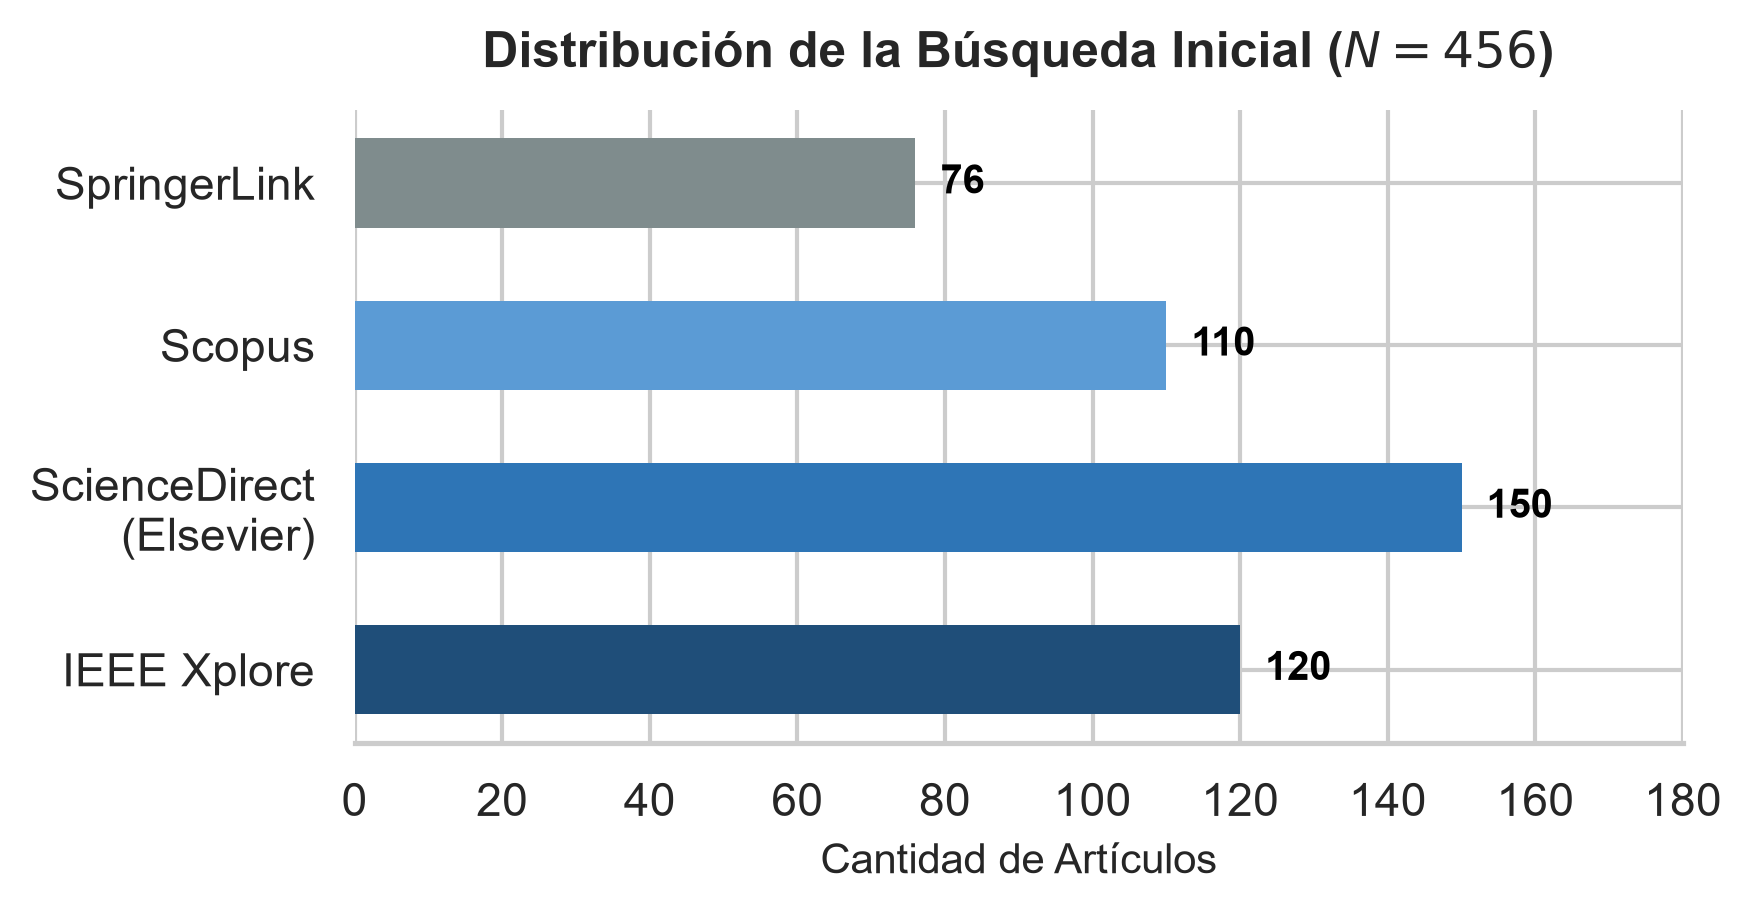
\includegraphics[width=0.48\textwidth]{../graficos/24_prisma_db_dist.png}}
\caption{Distribución de Artículos Encontrados en la Búsqueda Inicial por Base de Datos.}
\label{fig:db_dist}
\end{figure}

\subsection{Preguntas de Investigación y Enfoque PICO}
Para estructurar formalmente el alcance de la revisión sistemática, se formularon los objetivos bajo el marco conceptual PICO (Población, Intervención, Comparación y Resultado/Outcome), el cual se resume en la Tabla~\ref{tab:pico}.

\begin{table}[htbp]
\centering
\renewcommand{\arraystretch}{1.3}
\caption{Estructura del Enfoque PICO de la Revisión}
\label{tab:pico}
\begin{tabular}{@{}p{2.2cm}p{6.2cm}@{}}
\toprule
\textbf{Componente PICO} & \textbf{Descripción} \\
\midrule
\textbf{P}oblación / Contexto & Conductores viales y flujos de tráfico en entornos urbanos y autopistas. \\
\textbf{I}ntervención / Tecnología & Algoritmos de IA y Visión Computacional (Deep Learning, YOLO, CNNs, etc.). \\
\textbf{C}omparación & Enfoques metodológicos (DL, ML, Híbrido, OpenCV) y entornos (CCTV, UAV, Simulador, Vía Real). \\
\textbf{O}utcome (Resultado) & Métricas de desempeño (Accuracy, mAP), latencia (FPS) y viabilidad de despliegue (Edge Computing). \\
\bottomrule
\end{tabular}
\end{table}

Para guiar la recopilación y el análisis cuantitativo de la literatura, se plantearon tres preguntas de investigación fundamentales:
\begin{itemize}
    \item \textbf{PI1:} ¿Cuáles son las principales arquitecturas y enfoques metodológicos de Inteligencia Artificial y Visión por Computadora utilizados para el Monitoreo del Comportamiento de Conductores y los Sistemas de Transporte Inteligentes (ITS) en la literatura científica reciente (2020--2026)?
    \item \textbf{PI2:} ¿Qué entornos experimentales de prueba, plataformas de hardware de despliegue y herramientas de software de implementación predominan en la validación de estas tecnologías viales?
    \item \textbf{PI3:} ¿Cuáles son las limitaciones operativas, sesgos de datos y desafíos técnicos más críticos reportados por los investigadores, y qué direcciones de trabajo futuro se proponen para superarlos?
\end{itemize}

\subsection{Distribución Temporal de las Publicaciones}
El interés investigativo en la convergencia de la inteligencia artificial y el transporte inteligente ha mostrado una trayectoria de crecimiento significativo durante el periodo evaluado (2020--2026). Como se detalla en la Tabla~\ref{tab:dist_anos}, la cantidad de publicaciones anuales experimentó un incremento sostenido, alcanzando su pico de producción científica en el periodo 2024--2025 con un total de 97 trabajos. Este dinamismo refleja la rápida adopción de nuevas arquitecturas de aprendizaje profundo y la disponibilidad de hardware de bajo costo. La Fig.~\ref{fig:linea_publicaciones} ilustra visualmente esta tendencia de crecimiento en el volumen de publicaciones.

\begin{figure}[htbp]
\centerline{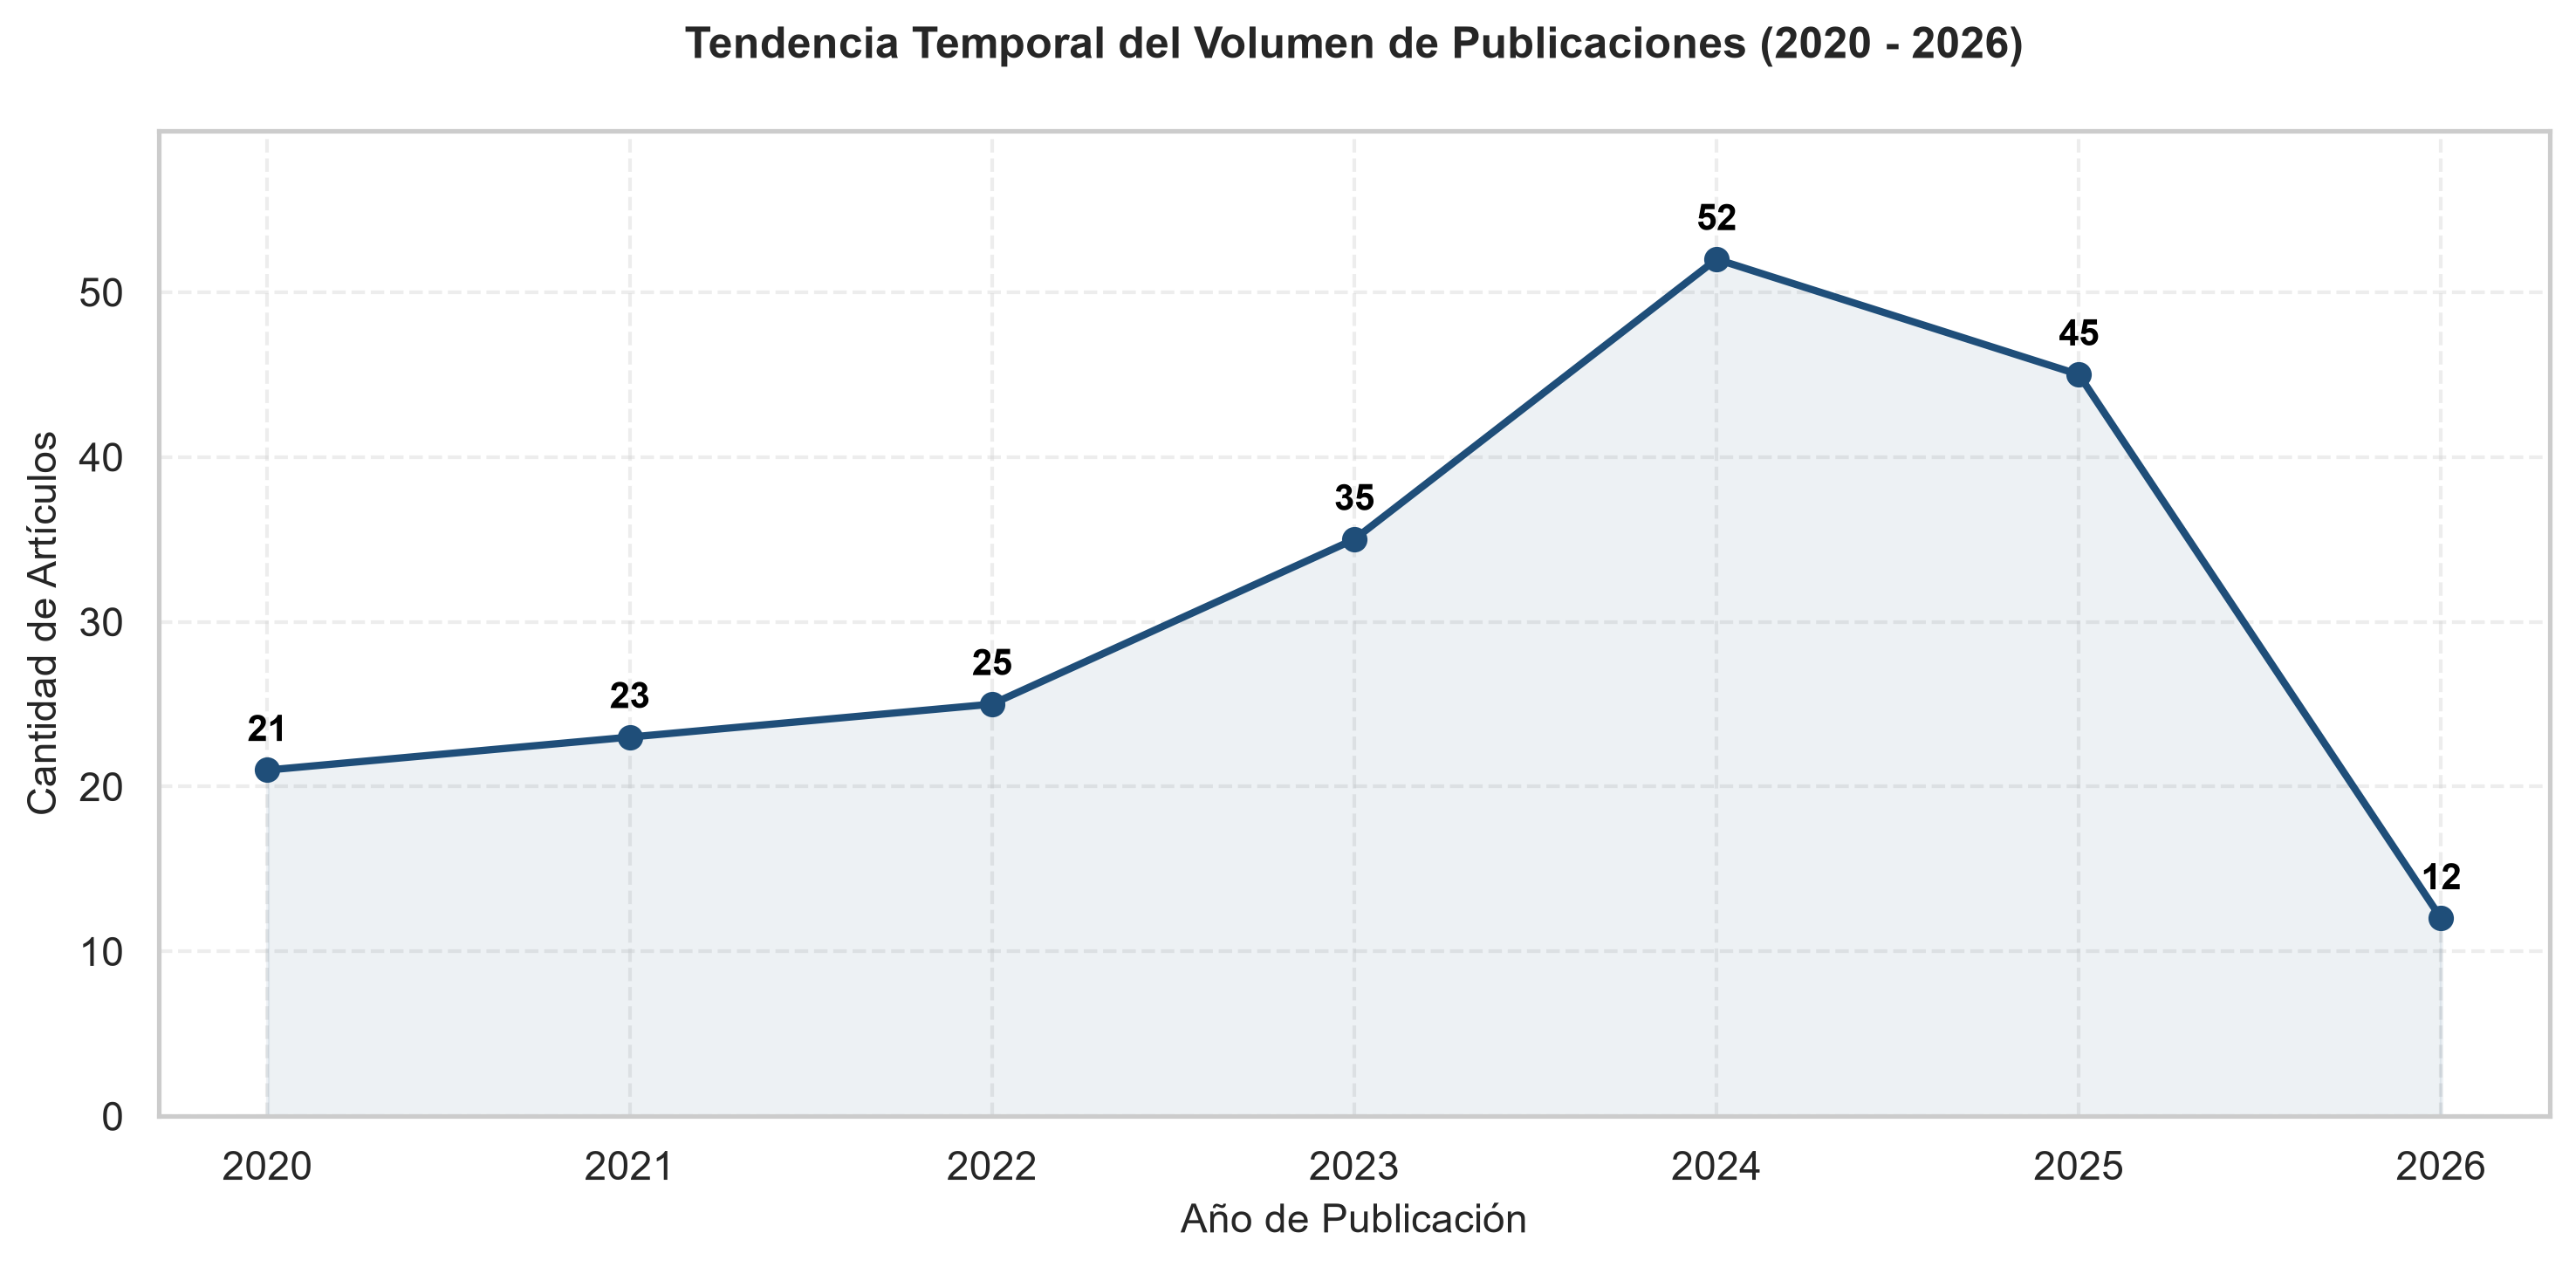
\includegraphics[width=0.48\textwidth]{../graficos/23_linea_publicaciones_año.png}}
\caption{Línea de Tendencia: Volumen Temporal de Publicaciones Científicas (2020--2026).}
\label{fig:linea_publicaciones}
\end{figure}

\begin{table}[htbp]
\centering
\renewcommand{\arraystretch}{1.2}
\caption{Distribución de Publicaciones Analizadas por Año}
\label{tab:dist_anos}
\begin{tabular}{cc}
\toprule
\textbf{Año de Publicación} & \textbf{Cantidad de Artículos} \\
\midrule
2020 & 21 \\
2021 & 23 \\
2022 & 25 \\
2023 & 35 \\
2024 & 52 \\
2025 & 45 \\
2026 & 12 \\
\bottomrule
\end{tabular}
\end{table}


Este crecimiento exponencial se alinea con la maduración de los frameworks de programación de deep learning como PyTorch y TensorFlow, que han facilitado enormemente la experimentación y despliegue rápido de modelos de visión compleja por parte de grupos de investigación en todo el mundo.

\subsection{Canales de Difusión y Venues Principales}
El análisis de los canales de publicación revela un corpus altamente consolidado en publicaciones de calidad. De los 213 artículos analizados, 175 corresponden a artículos de revistas científicas de alto impacto (journals) y 38 a contribuciones presentadas en conferencias internacionales de prestigio, destacando la marcada presencia de revistas líderes en el área como \textit{IEEE Transactions on Intelligent Transportation Systems} y \textit{Sensors}. La concentración en estas revistas y congresos especializados subraya la solidez científica del corpus analizado y asegura la relevancia técnica de las tendencias estadísticas y metodológicas que se derivan de la presente revisión.

\subsection{Clasificación de Enfoques de Inteligencia Artificial}
Para analizar la evolución de las técnicas de IA, los artículos han sido clasificados en cuatro categorías principales basadas en la descripción de sus algoritmos:
\begin{itemize}
    \item \textbf{Deep Learning (DL):} Trabajos fundamentados en redes neuronales convolucionales (CNN), modelos YOLO, redes de memoria a largo y corto plazo (LSTM) y arquitecturas de Transformers de visión (ViT), representando la gran mayoría de las propuestas debido a su capacidad para procesar datos no estructurados de alta dimensión.
    \item \textbf{Machine Learning (ML):} Algoritmos tradicionales de aprendizaje automático como máquinas de soporte vectorial (SVM), bosques aleatorios (Random Forest), K-vecinos cercanos (KNN) o modelos bayesianos.
    \item \textbf{Híbrido (ML + DL):} Estudios que integran representaciones de características de Deep Learning con clasificadores tradicionales de Machine Learning para optimizar el rendimiento y reducir el tiempo de entrenamiento.
    \item \textbf{Visión por Computadora Tradicional:} Propuestas basadas puramente en procesamiento de imágenes digital básico o descriptores geométricos mediante librerías como OpenCV tradicional sin el entrenamiento de modelos predictivos complejos.
\end{itemize}

La Tabla~\ref{tab:dist_metodologias} detalla la distribución cuantitativa de estos enfoques dentro del corpus.

\begin{table}[htbp]
\centering
\renewcommand{\arraystretch}{1.2}
\caption{Distribución por Enfoque Metodológico}
\label{tab:dist_metodologias}
\begin{tabular}{lc}
\toprule
\textbf{Enfoque Metodológico} & \textbf{Cantidad de Artículos} \\
\midrule
Deep Learning (DL) & 135 \\
Otros / No especificado & 44 \\
Híbrido (ML + DL) & 23 \\
Machine Learning (ML) & 11 \\
\bottomrule
\end{tabular}
\end{table}


La Fig.~\ref{fig:cruce_metodologias_entornos} ilustra la correlación existente entre los enfoques metodológicos adoptados y los entornos experimentales en los que se validan las soluciones. Como se aprecia, existe una clara preferencia por validar los modelos de Deep Learning en entornos de CCTV y escenarios reales de vía pública.

\begin{figure}[htbp]
\centerline{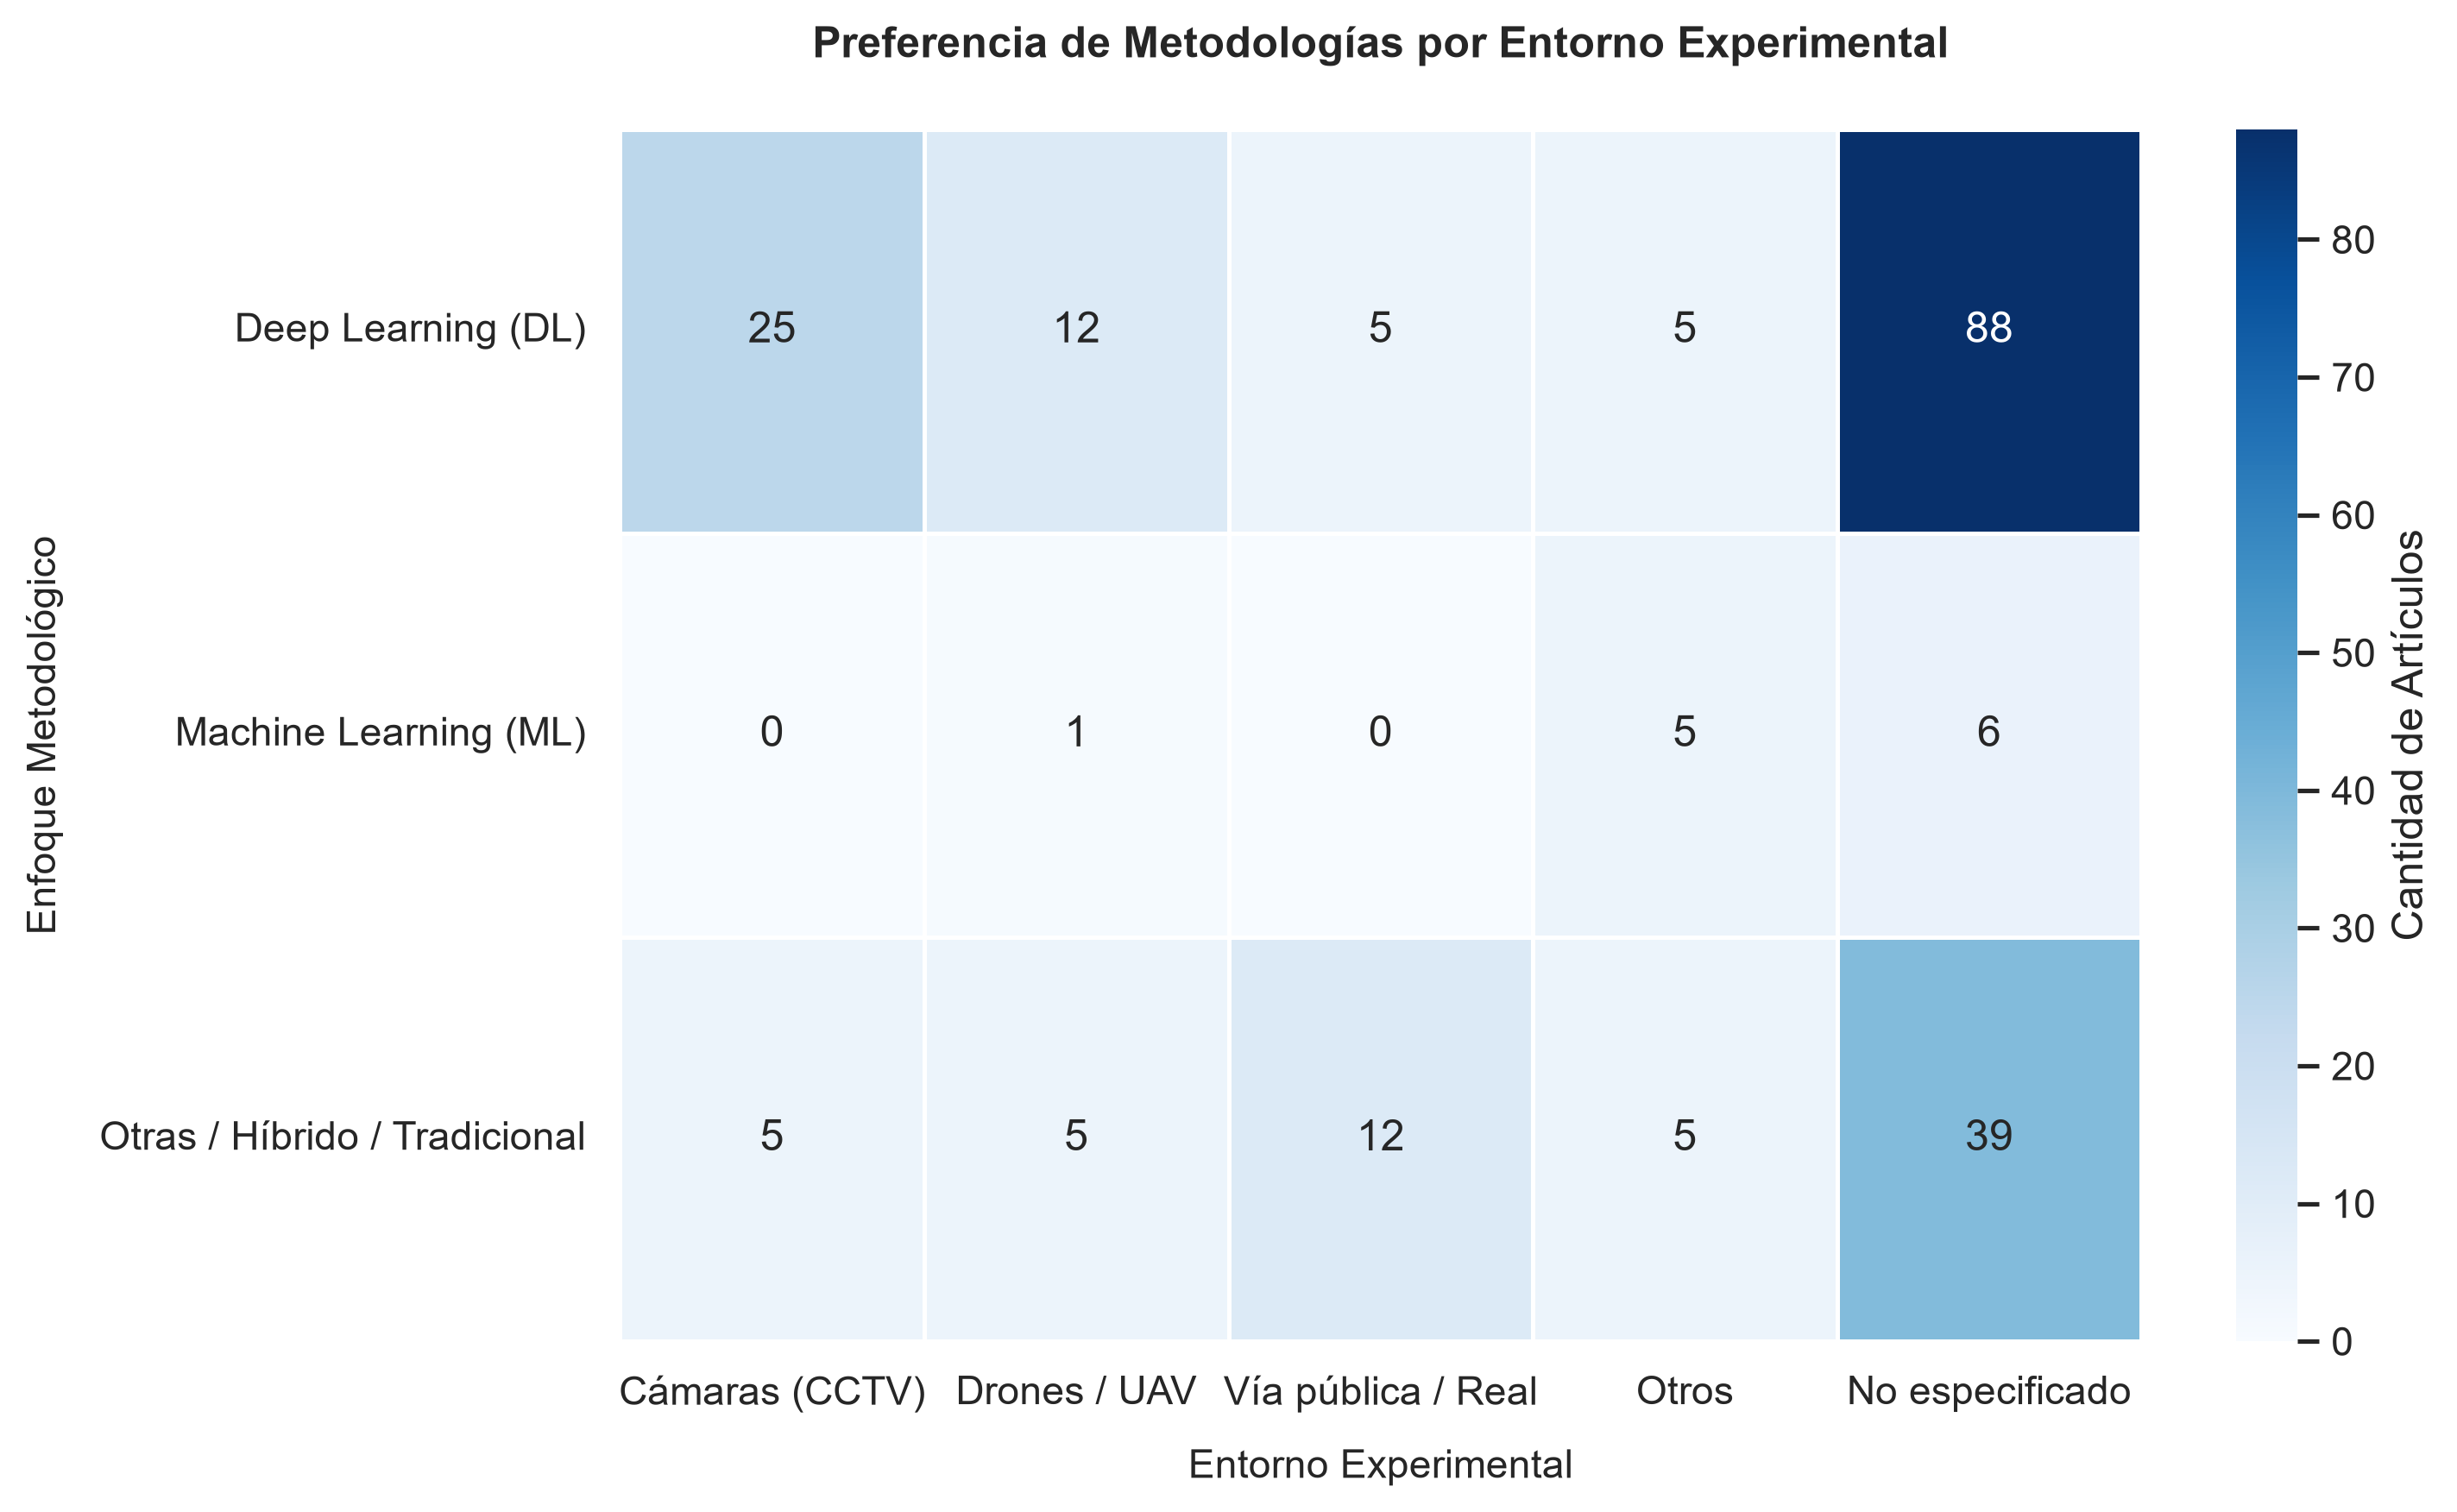
\includegraphics[width=0.48\textwidth]{../graficos/16_heatmap_cruce_3x3_entornos.png}}
\caption{Preferencia de Metodologías por Entorno Experimental (Distribución porcentual).}
\label{fig:cruce_metodologias_entornos}
\end{figure}

\section{Resultados}
El análisis detallado del corpus literario revela las tendencias tecnológicas que definen la frontera del conocimiento en ITS y monitoreo de conductores, exponiendo una clara transición metodológica desde modelos matemáticos deterministas hacia sistemas adaptativos de redes neuronales profundas.

\subsection{Dominio de Algoritmos YOLO en Tareas de Detección}
Dentro del paradigma de Deep Learning, las arquitecturas de detección de objetos en una sola etapa (one-stage detectors) dominan la literatura de forma abrumadora debido a su capacidad de inferencia en tiempo real. Específicamente, los modelos de la familia YOLO (You Only Look Once) son la primera opción para tareas de detección en tiempo real de vehículos e infracciones. Los modelos YOLOv5 \cite{kumar2026uavbased, chen2026hybrid} continúan siendo ampliamente referenciados y adaptados debido a su madurez y facilidad de entrenamiento. Para tareas de vigilancia de tráfico a gran escala, variantes optimizadas de YOLOv5 \cite{zia2025advancing, yang2025computer} logran excelentes tasas de detección de camiones y motocicletas. Asimismo, estudios centrados en la compresión de modelos \cite{essahraui2025realtime, jing2025traffic} demuestran que la cuantización de pesos viabiliza su ejecución en hardware con recursos limitados.

Paralelamente, YOLOv8 \cite{pavan2026aipowered, essahraui2025realtime} se consolida como la arquitectura preferida para aplicaciones que demandan un alto balance entre velocidad y precisión, incorporando innovaciones como la cabeza de detección libre de anclajes (anchor-free) y una estructura de pérdida modificada. Varios investigadores han propuesto mejoras a la capa de atención de YOLOv8 \cite{satya2025utilization, le2025redlight} para mitigar la tasa de falsos negativos en condiciones de lluvia o niebla. Otros trabajos \cite{silva2025light, oussouaddi2025dsryolo} integran YOLOv8 con estimadores de velocidad basados en flujo óptico. Asimismo, versiones más recientes e híbridas como YOLOv7 \cite{liu2026research, alshehri2025integrated}, YOLOv9 \cite{xie2025yoloace}, YOLOv10  y YOLOv11  demuestran innovaciones en términos de eficiencia de parámetros y atención multiescala, permitiendo capturar vehículos a gran distancia en tomas de alta resolución espacial.

Asimismo, investigaciones muy recientes comienzan a explorar la transición desde detectores de objetos basados puramente en convoluciones hacia arquitecturas basadas en Transformers de tiempo real, tales como RT-DETR \cite{yang2025computer, essahraui2025realtime}. Estos modelos eliminan la necesidad del procesamiento posterior de Supresión No Máxima (NMS, por sus siglas en inglés), el cual suele representar un cuello de botella de latencia crítico en sistemas embebidos de tráfico cuando la densidad de vehículos es extremadamente alta \cite{lin2025dangerous, satya2025utilization}. Al procesar las relaciones espaciales mediante auto-atención multi-escala directa de manera paralela, RT-DETR y sus variantes híbridas prometen un rendimiento de detección más estable frente a oclusiones mutuas de vehículos en autopistas saturadas, abriendo una nueva línea de optimización para los sistemas inteligentes de transporte de próxima generación.

\subsection{Redes Neuronales Convolucionales y Modelos Temporales}
Las redes convolucionales clásicas (CNN) \cite{liu2026research, zambrano2026monitoring} se mantienen como la base estructurante para el análisis de fatiga y la clasificación fina de expresiones faciales a través de marcas faciales. Para robustecer la detección frente a cambios rápidos en la pose de la cabeza, se proponen redes CNN multirrama \cite{l2026safestreets, ahmad2026comparative} y modelos basados en MobileNet \cite{chen2026hybrid, zia2025advancing} optimizados para bajo consumo energético. 

Para la modelación temporal de secuencias de video (por ejemplo, el análisis continuo del comportamiento o de colisiones a lo largo del tiempo), los autores recurren a redes recurrentes y LSTM \cite{kumar2026intelligent, ahmad2026comparative}. Las arquitecturas combinadas CNN-LSTM \cite{alshehri2025integrated, ijaradar2025datadriven} permiten capturar transiciones dinámicas como el pestañeo lento o el cabeceo del conductor. Otros desarrollos \cite{duan2025multimodal, arjunan2024realtime} aplican redes de memoria para la predicción de trayectorias vehiculares en cruces urbanos. Por último, la irrupción de los Vision Transformers (ViT) y mecanismos de auto-atención \cite{kumar2026intelligent, lin2025dangerous} marca un cambio tecnológico relevante, permitiendo capturar relaciones espaciotemporales de largo alcance con mayor precisión. Modelos espaciotemporales basados en atención \cite{huang2025dtldetector, alshehri2025integrated} y transformers de escala temporal \cite{kumar2025smart, tran2024transformerbased} se posicionan como alternativas altamente precisas aunque computacionalmente costosas.

\subsection{Enfoques de Machine Learning y Arquitecturas Híbridas}
A pesar del dominio del aprendizaje profundo, los algoritmos tradicionales de Machine Learning mantienen un rol importante en el estado del arte. Los modelos SVM \cite{abarghooei2026driving, ahmad2026comparative} y Random Forest \cite{uddin2025abnormal, usman2024distracted} se emplean comúnmentmente para la clasificación final de datos tabulares provenientes de sensores a bordo del vehículo o variables fisiológicas directas. Adicionalmente, clasificadores tradicionales \cite{essahraui2025realtime, wu2024driving} y modelos basados en árboles \cite{xue2023young, dong2022fatigue} ofrecen una alta interpretabilidad requerida para sistemas de seguridad activa críticos.

Adicionalmente, las arquitecturas híbridas \cite{ahmad2026comparative, essahraui2025realtime} combinan el poder de representación de características de Deep Learning (usando CNNs como extractores automáticos de características de alto nivel) con la robustez estadística de los clasificadores ML tradicionales para reducir la latencia de inferencia y optimizar el rendimiento en hardware de borde con recursos limitados. Propuestas basadas en la extracción híbrida \cite{mota2025integration, suresh2025traffic} reducen el tiempo de entrenamiento sin sacrificar precisión. Por su parte, los enfoques tradicionales de visión por computadora  se aplican en la etapa de preprocesamiento, como la normalización del contraste y la segmentación básica de regiones de interés (ROI) mediante umbralización y descriptores geométricos básicos .

\subsection{Entornos Experimentales de Prueba y Despliegue de Hardware}
Los entornos experimentales reportados en la literatura científica para validar estas soluciones inteligentes se clasifican en cuatro áreas principales:
\begin{enumerate}
    \item \textbf{Cámaras de Videovigilancia (CCTV):} Utilizadas principalmente para el monitoreo pasivo de intersecciones urbanas, detección de infracciones y detección automática de colisiones \cite{l2026safestreets, kumar2026intelligent}.
    \item \textbf{Cámaras A bordo / Conducción Naturalista:} Conducción en vehículos reales o simuladores con cámaras de cabina \cite{liu2026research, rahman2026costeffective}.
    \item \textbf{Imágenes Aéreas (UAV / Drones):} Toma aérea de tráfico y trayectorias \cite{kumar2026uavbased, bhavsar2025evaluating}.
    \item \textbf{Simuladores de Conducción / Entornos Virtuales:} Simuladores en PC o cabinas virtuales \cite{abarghooei2026driving, zambrano2026monitoring}.
\end{enumerate}

Para profundizar en las relaciones entre el entorno experimental y las librerías o hardware utilizados, la Fig.~\ref{fig:heatmap_relacion} ilustra la concentración de trabajos mediante un mapa de calor coincidente de frecuencias. Como se observa, existe una fuerte dependencia del uso de librerías como OpenCV o MediaPipe aplicadas sobre entornos reales y CCTV \cite{ahmad2026comparative, srivastava2026traffic}, mientras que el hardware de borde especializado como las GPUs NVIDIA Jetson y Raspberry Pi representan los principales habilitadores para implementar estos sistemas directamente en vehículos reales y UAV \cite{fei2025enhancing, zuo2025composite}.

\begin{figure}[htbp]
\centerline{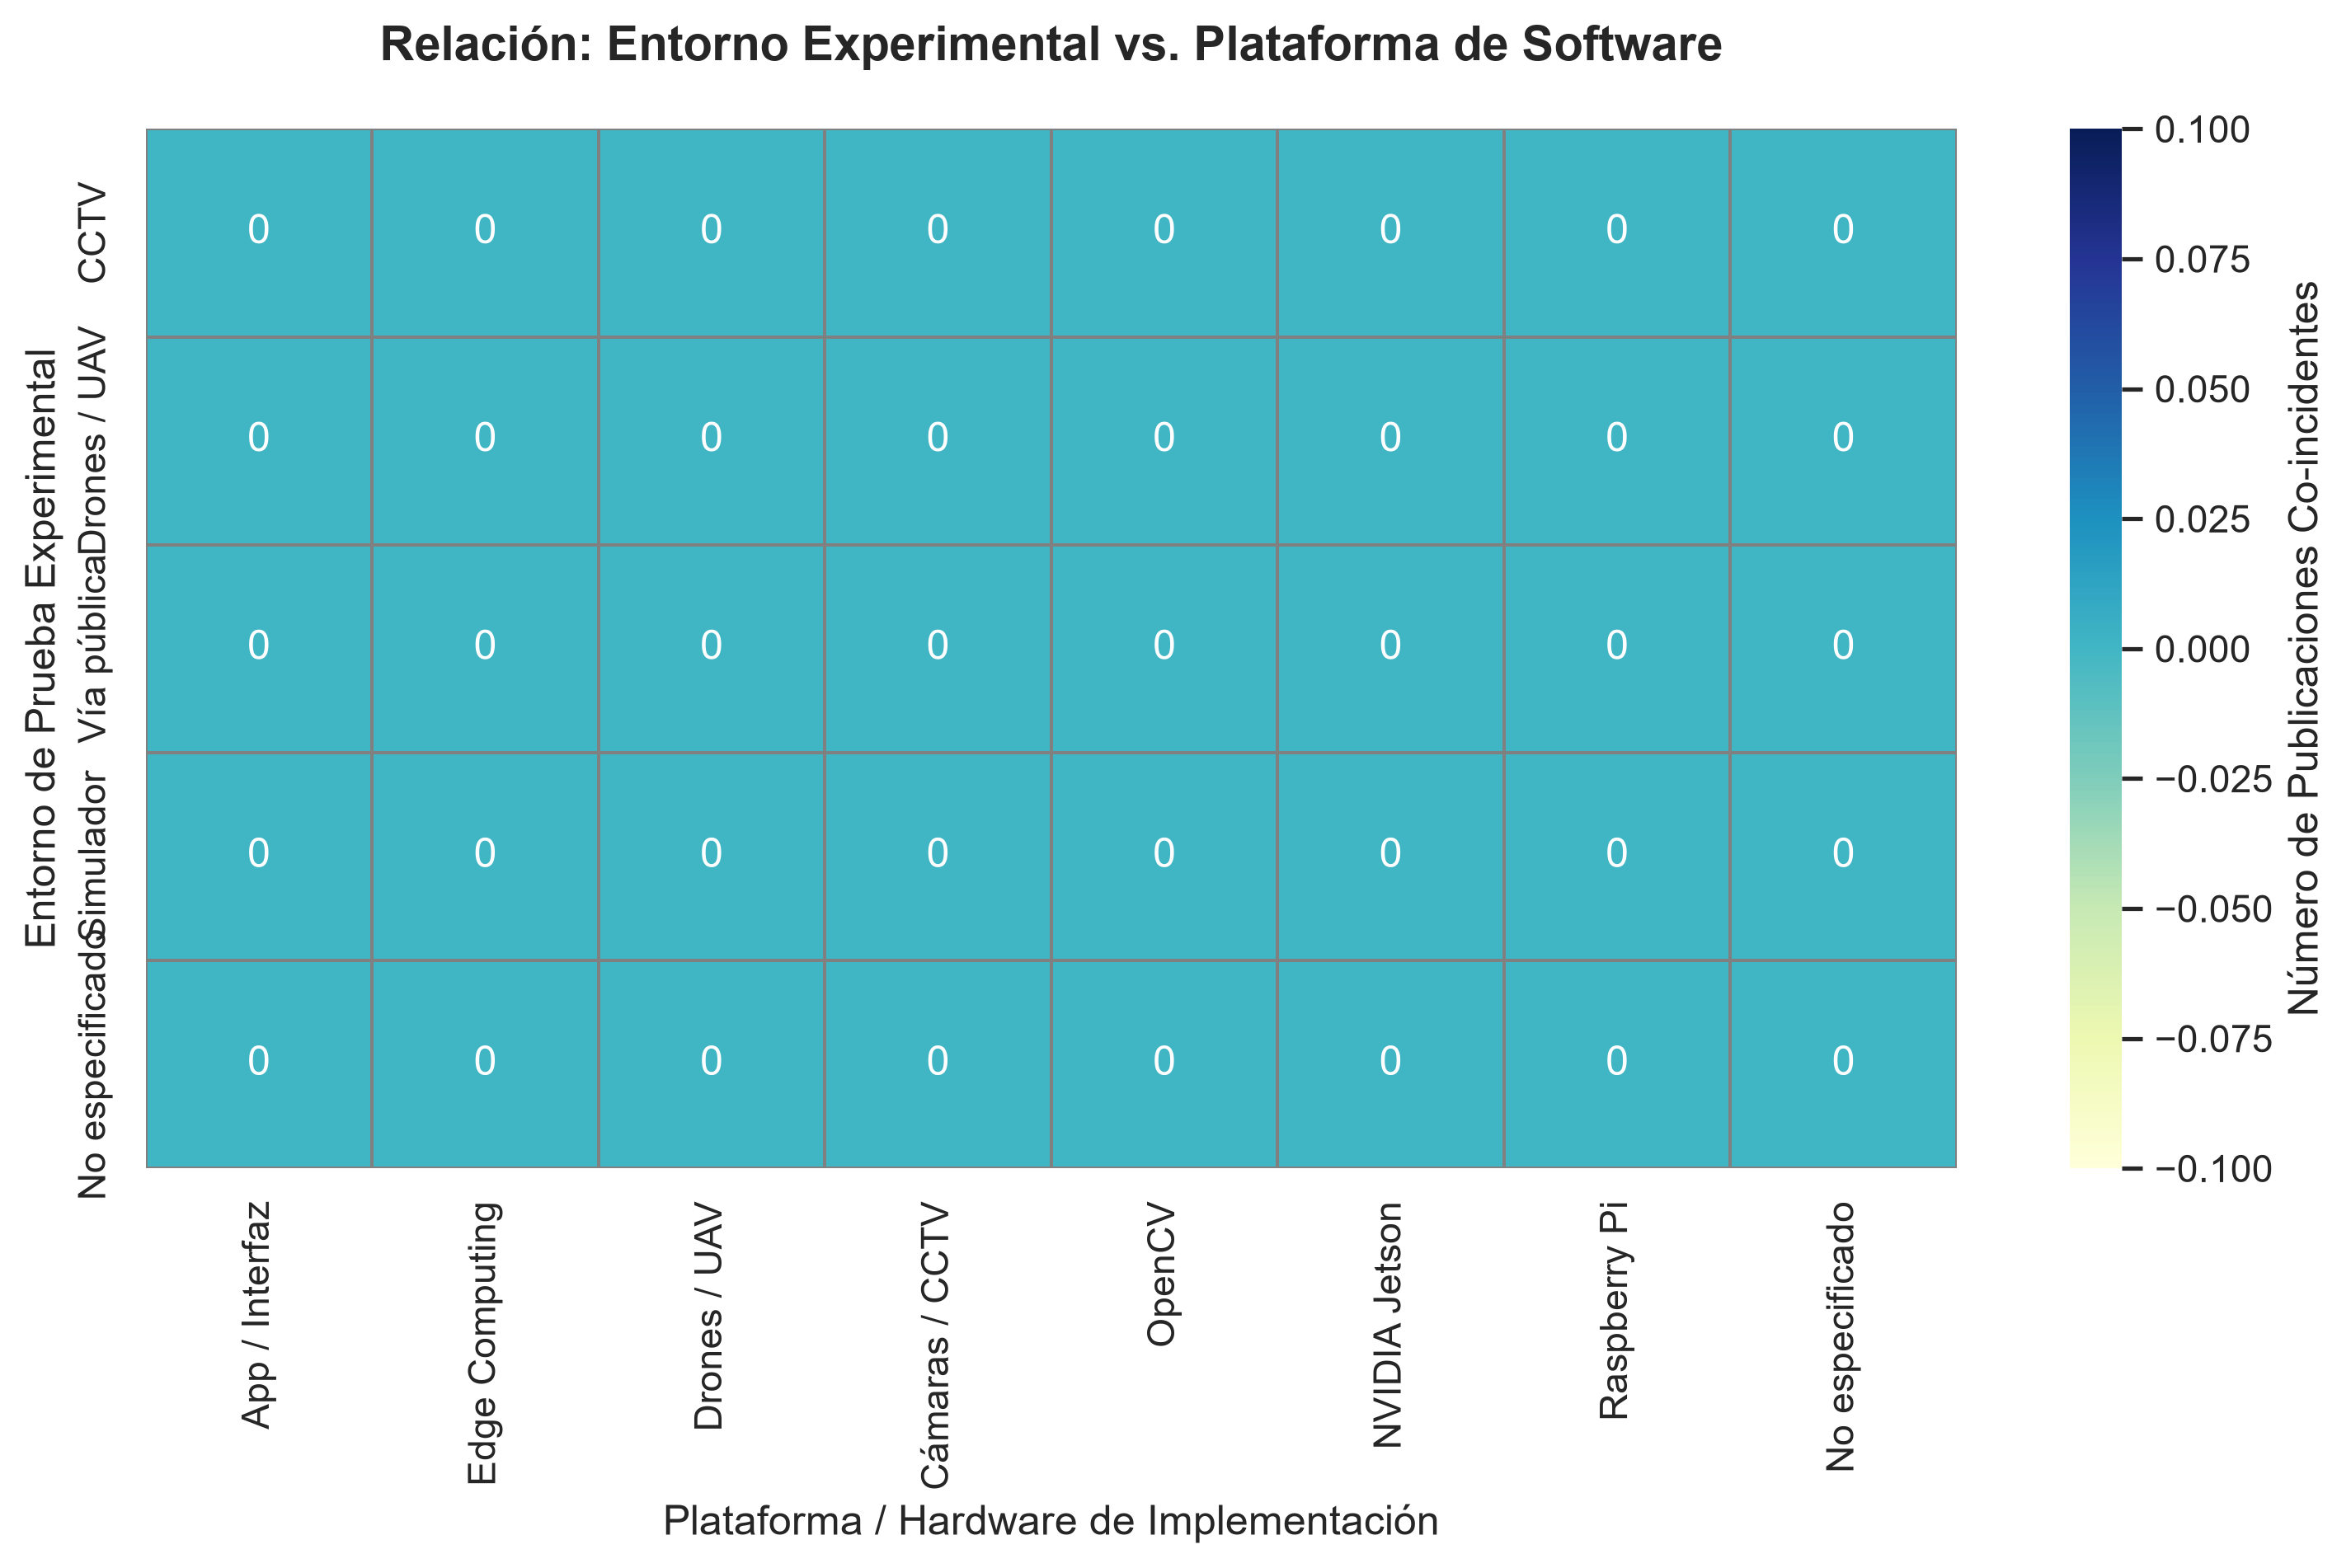
\includegraphics[width=0.48\textwidth]{../graficos/10_heatmap_relacion.png}}
\caption{Mapa de Calor Cruzado: Entorno Experimental vs. Plataforma de Implementación de Software y Hardware.}
\label{fig:heatmap_relacion}
\end{figure}

\begin{figure}[htbp]
\centerline{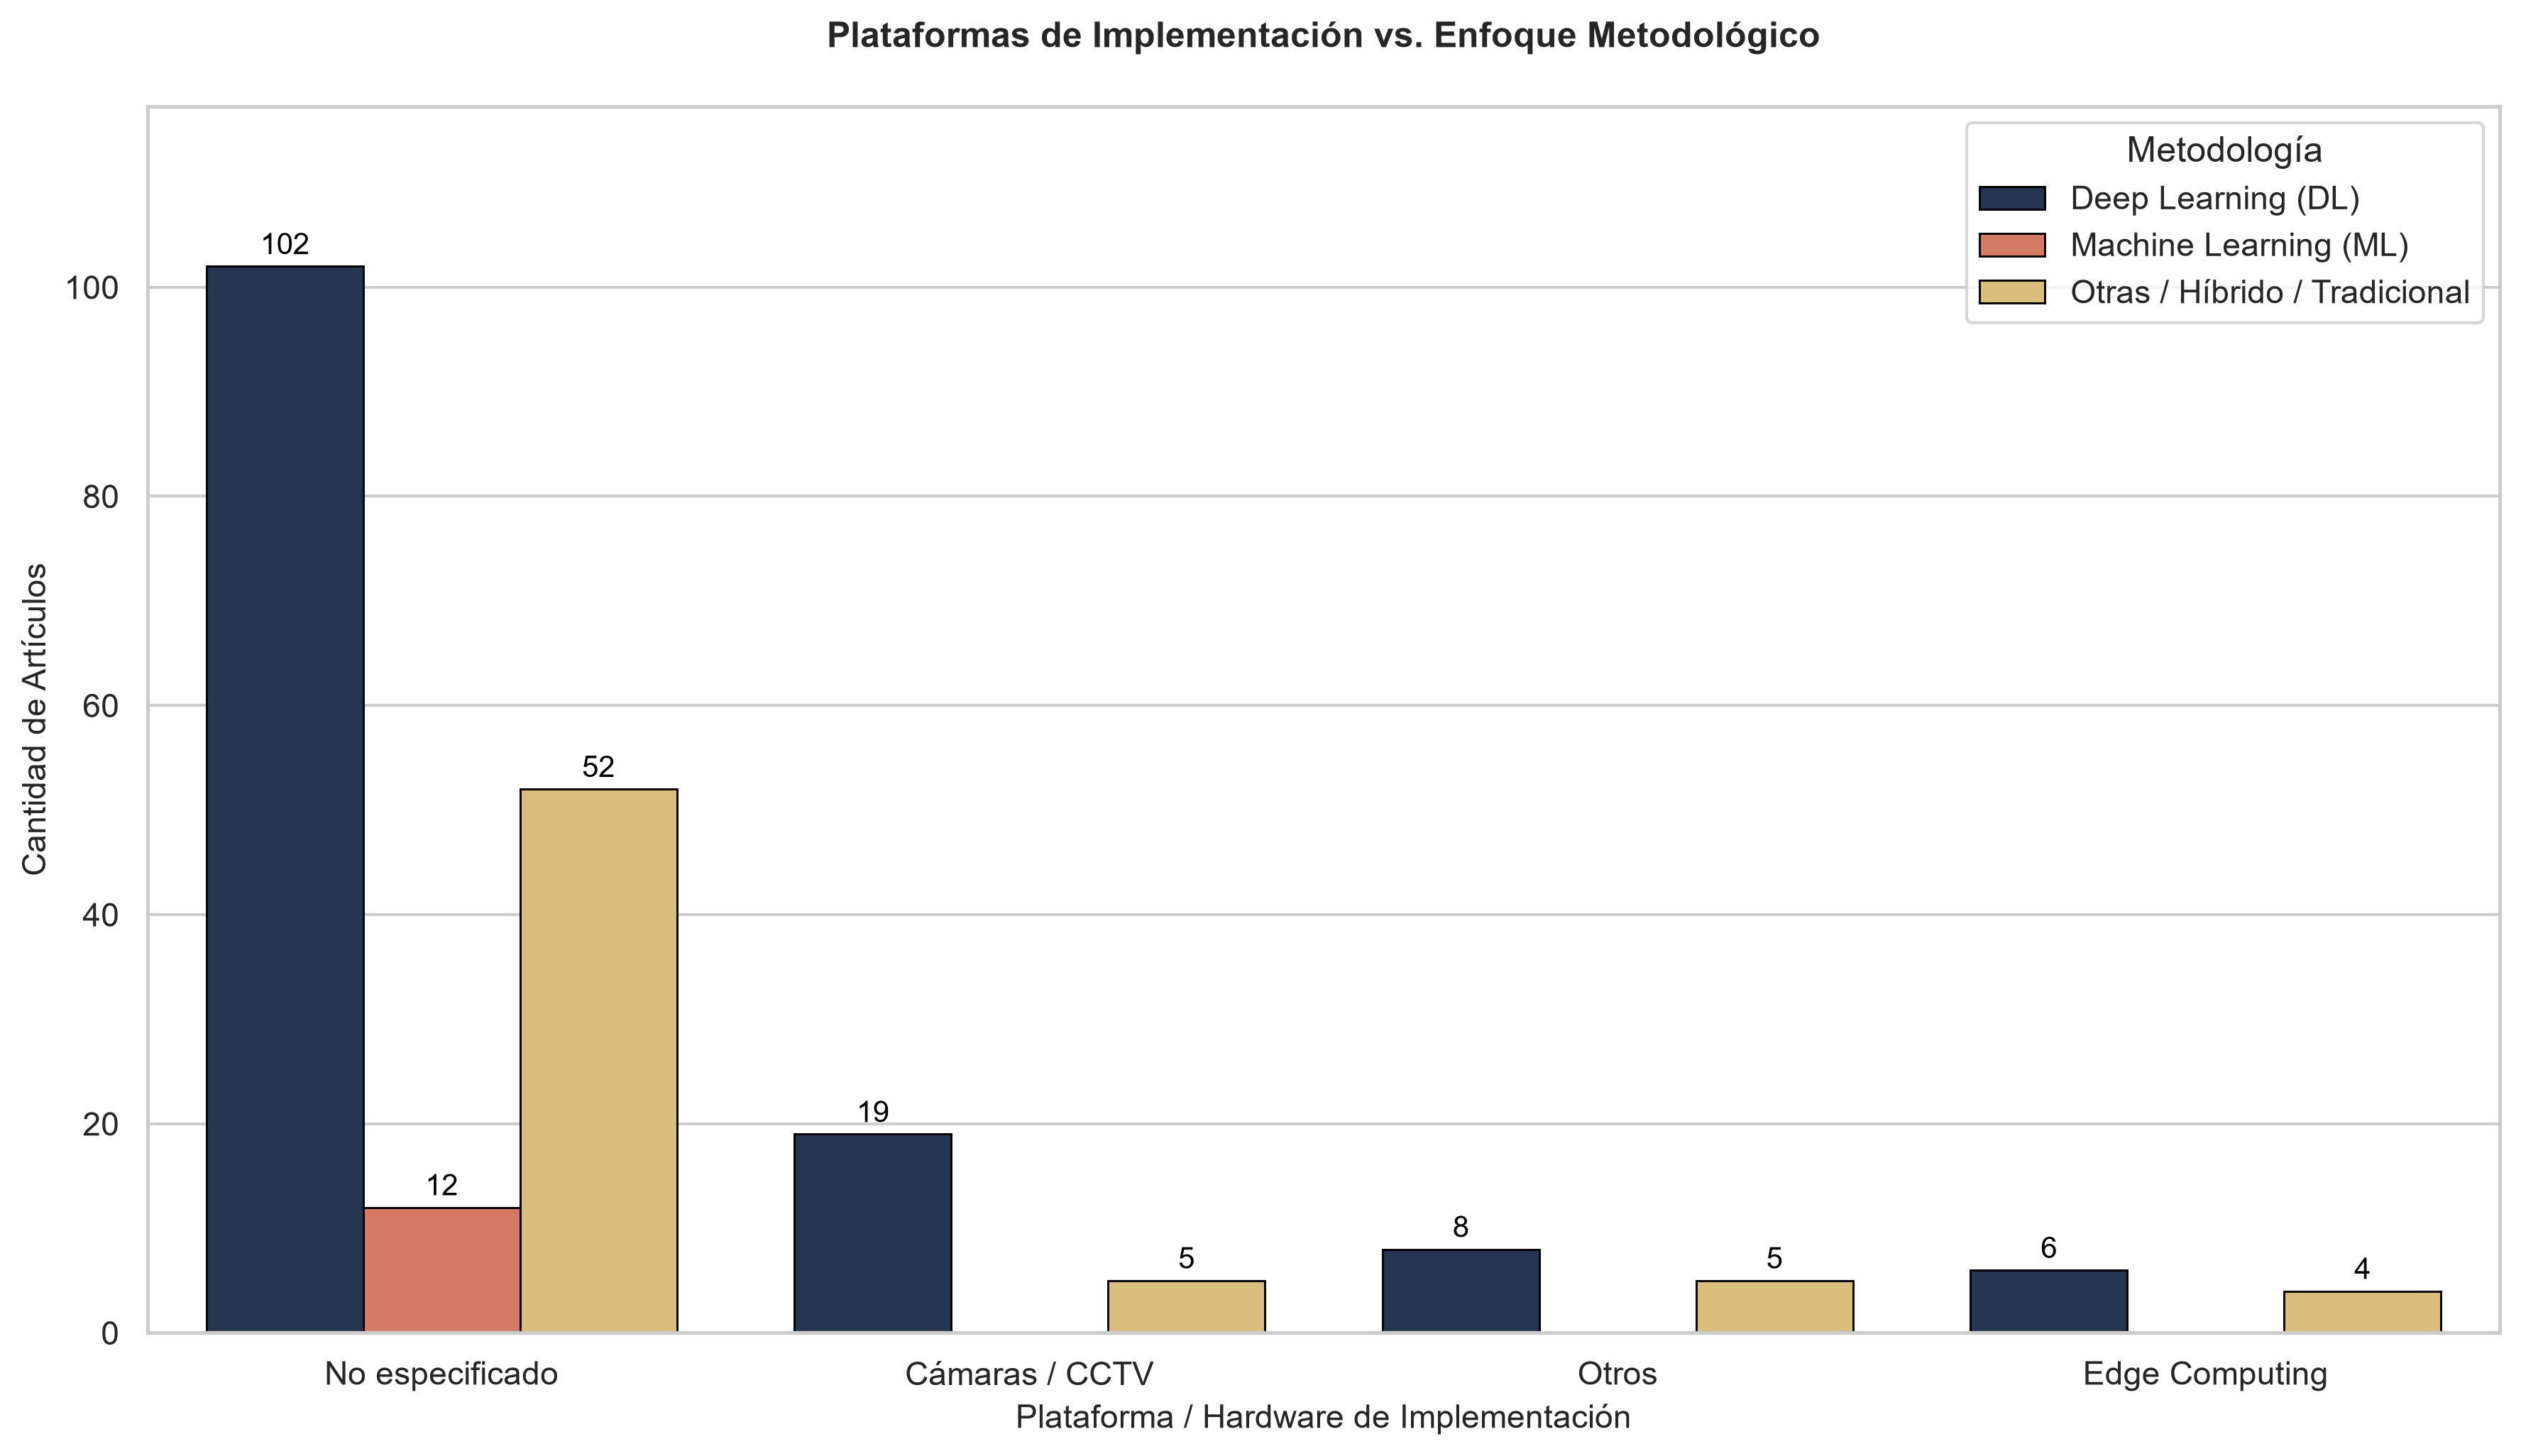
\includegraphics[width=0.48\textwidth]{../graficos/17_cruce_implementacion_metodologia.png}}
\caption{Plataformas de Implementación vs. Enfoque Metodológico de la Investigación.}
\label{fig:cruce_implementacion}
\end{figure}

\subsection{Evaluación del Rendimiento y Métricas Comparativas}
La evaluación del rendimiento de los modelos en la literatura científica se basa en métricas de clasificación y regresión bien establecidas en visión por computadora. Entre las principales se encuentran la exactitud (Accuracy), la precisión (Precision), la sensibilidad (Recall), el puntaje F1 (F1-Score) y la precisión media promedio (mAP). Las fórmulas que gobiernan estas métricas principales se definen de la siguiente manera:

\begin{equation}
\text{Accuracy} = \frac{\text{TP} + \text{TN}}{\text{TP} + \text{TN} + \text{FP} + \text{FN}}
\end{equation}

\begin{equation}
\text{Precision} = \frac{\text{TP}}{\text{TP} + \text{FP}}
\end{equation}

\begin{equation}
\text{Recall} = \frac{\text{TP}}{\text{TP} + \text{FN}}
\end{equation}

\begin{equation}
\text{F1-Score} = 2 \cdot \frac{\text{Precision} \cdot \text{Recall}}{\text{Precision} + \text{Recall}}
\end{equation}

donde TP representa los verdaderos positivos, TN los verdaderos negativos, FP los falsos positivos y FN los falsos negativos. Para evaluar cuantitativamente el desempeño de estas soluciones en base a la literatura que reporta métricas numéricas concretas, la Fig.~\ref{fig:boxplot_accuracy} expone mediante diagramas de caja y bigotes la distribución del rendimiento (\textit{accuracy}) reportado según el enfoque metodológico de IA empleado. Este análisis comparativo consolida visualmente la efectividad del aprendizaje profundo en contraste con otras aproximaciones estadísticas o híbridas \cite{fei2025enhancing, jing2025traffic}.

\begin{figure}[htbp]
\centerline{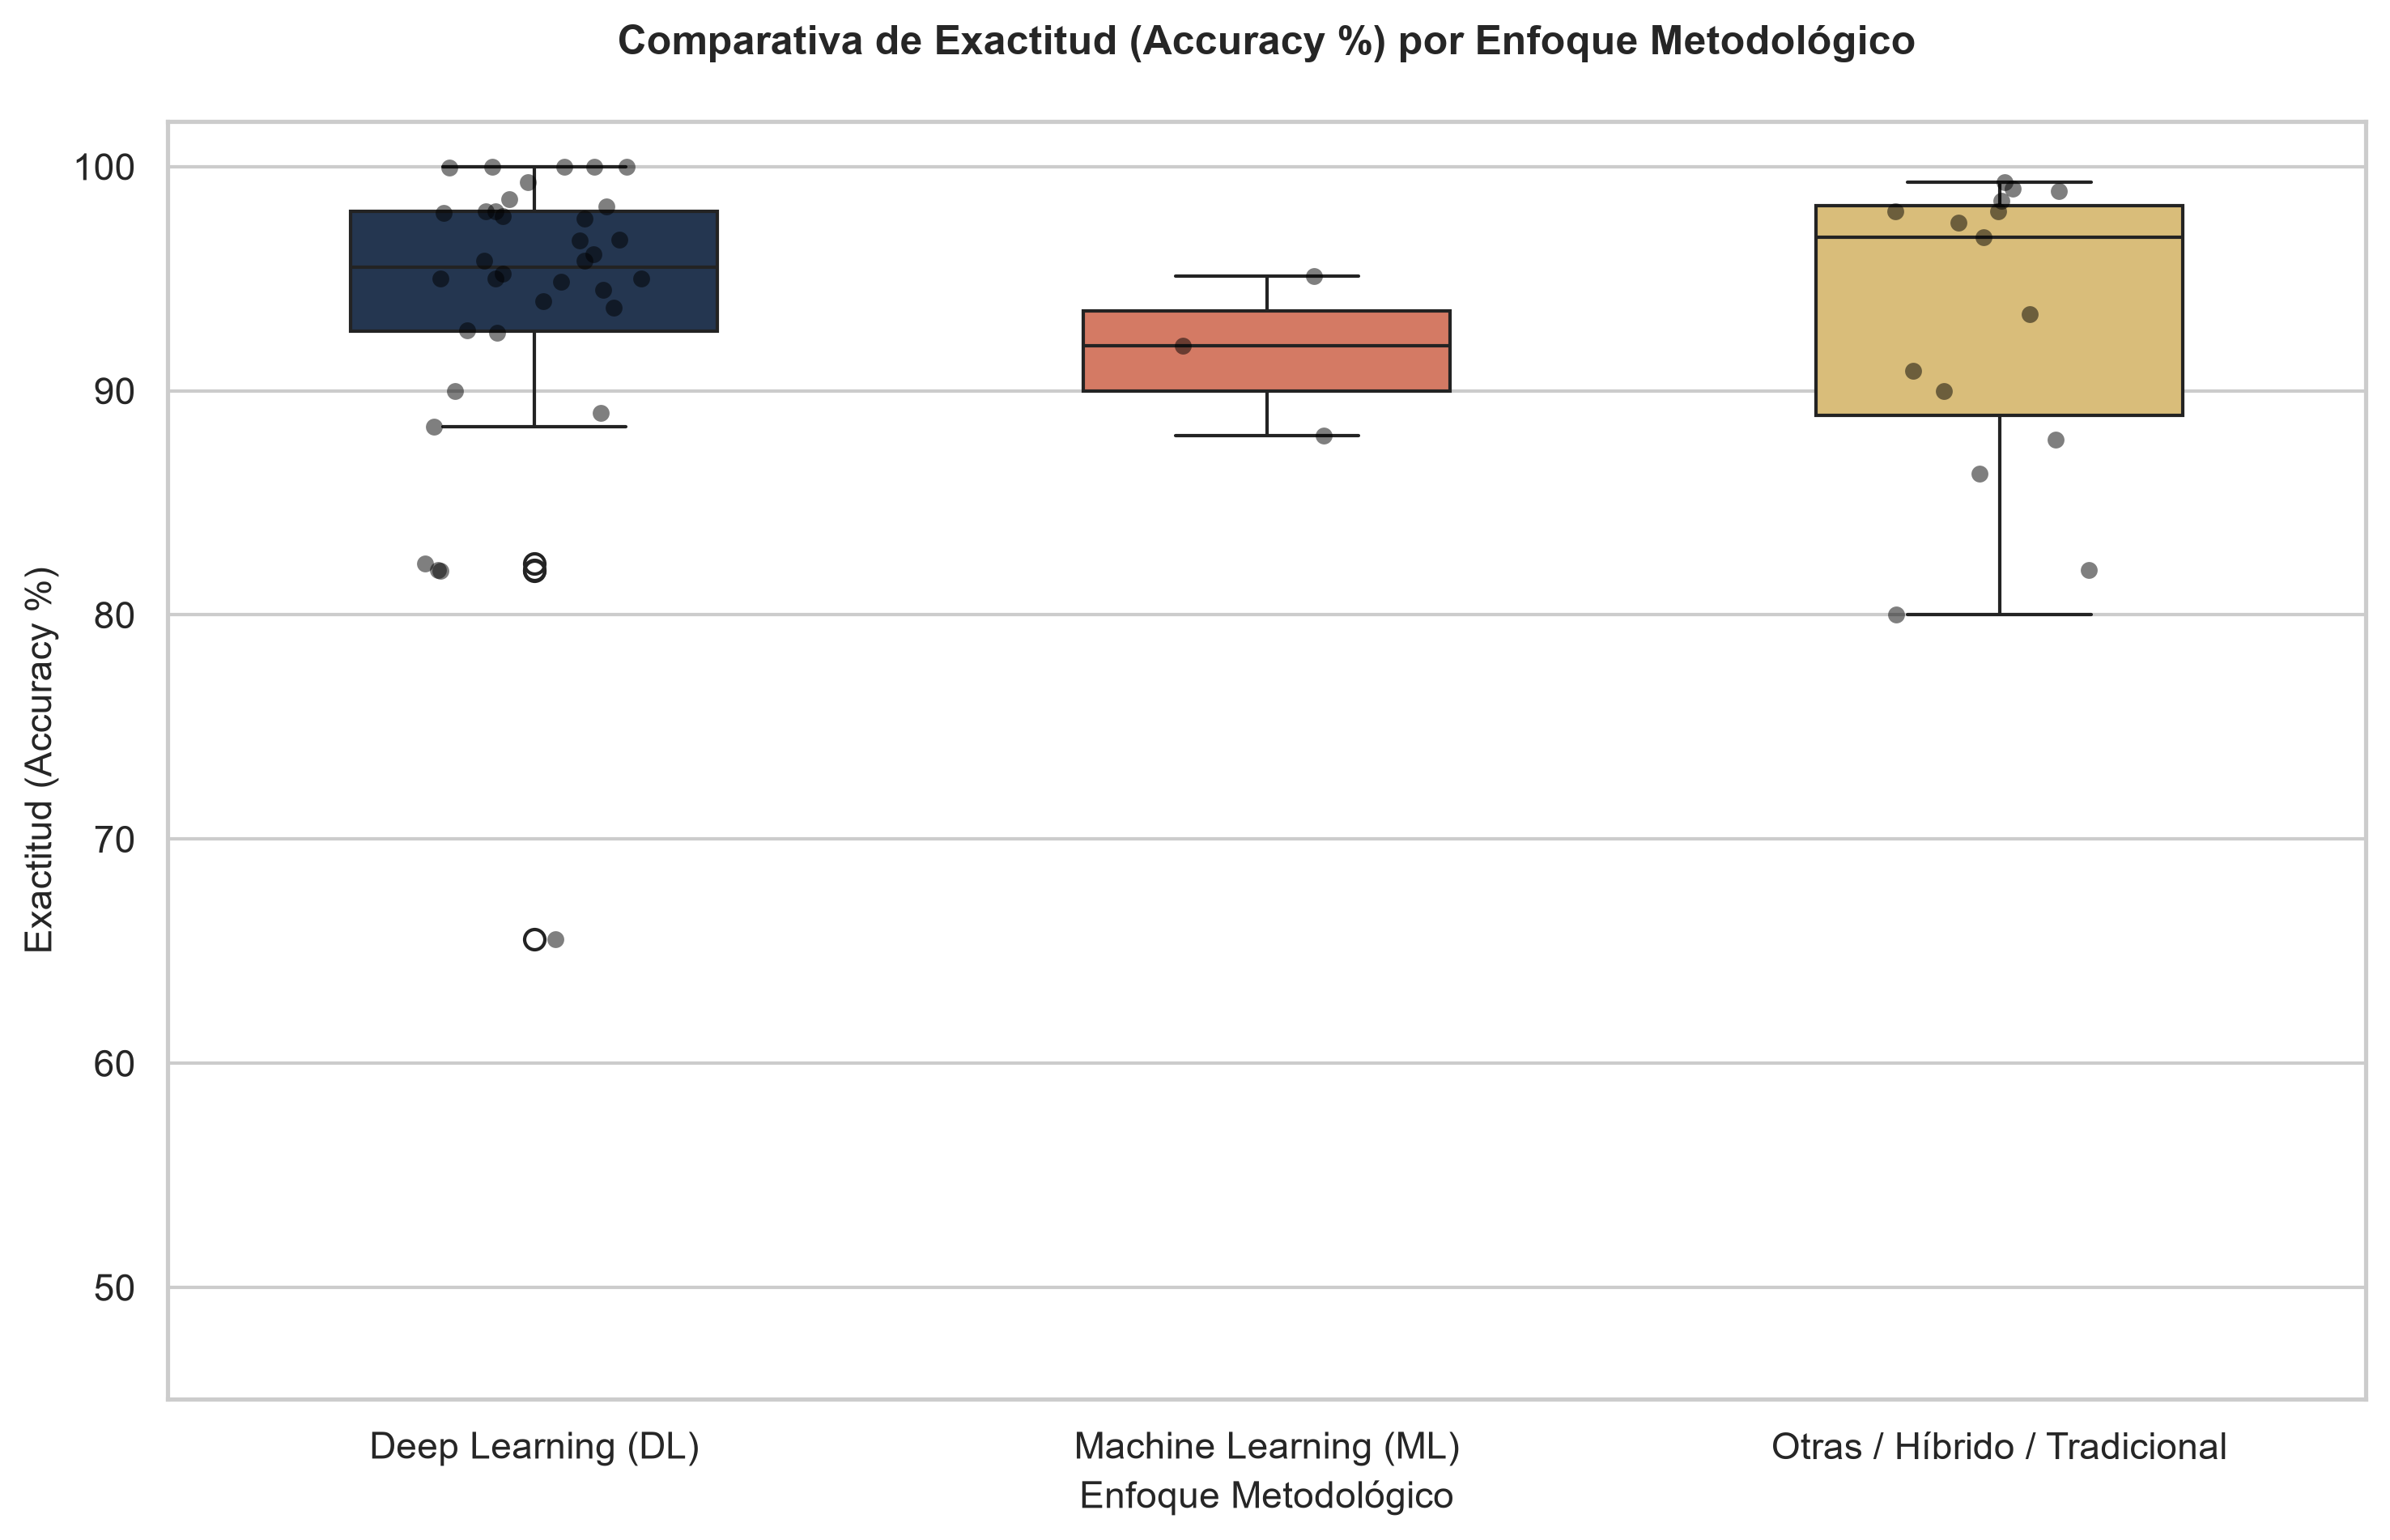
\includegraphics[width=0.48\textwidth]{../graficos/20_boxplot_accuracy_metodologia.png}}
\caption{Comparativa de la Distribución de Exactitud (Accuracy \%) según el Enfoque Metodológico de IA.}
\label{fig:boxplot_accuracy}
\end{figure}

\subsection{Tabulación de Investigaciones Destacadas}
Las Tablas de la \ref{tab:articulos_conductores_1} a la \ref{tab:articulos_conductores_4} y de la \ref{tab:articulos_transporte_1} a la \ref{tab:articulos_transporte_5} presentan el compendio total de las investigaciones analizadas en esta revisión sistemática, detallando la metodología de IA, el entorno experimental y las métricas de rendimiento de cada trabajo.

\begin{table*}[htbp]
\centering
\renewcommand{\arraystretch}{1.1}
\caption{Resumen de Investigaciones en Monitoreo de Conductores y Métricas de Rendimiento (Parte 1)}
\label{tab:articulos_conductores_1}
\footnotesize
\begin{tabular}{cp{7.5cm}p{2.8cm}p{2.8cm}p{2.8cm}}
\toprule
\textbf{Ref.} & \textbf{Título del Trabajo} & \textbf{Metodología IA} & \textbf{Entorno de Prueba} & \textbf{Métrica de Rendimiento} \\
\midrule
\cite{liu2026research} & Research on the Analysis and Recognition System for Dangerous Driving Behaviors Based o... & YOLOv11, CNN (Redes Convoluciona... & Conducción naturalista / Vehícul... & mAP50 of 69.26, accuracy of 65.5... \\
\cite{abarghooei2026driving} & Driving Behavior Classification and Risk Quantification via Multisensor Machine Learnin... & SVM, Machine Learning & Simulador de conducción / Entorn... & 92\% accuracy, 88\% accuracy \\
\cite{hu2026trustworthy} & Trustworthy Driver State Perception via Contextual Interaction-Driven Evidential Vision... & Deep Learning & No especificado & No especificado \\
\cite{zambrano2026monitoring} & Driver Monitoring System Using Computer Vision for Real-Time Detection of Fatigue, Dist... & CNN (Redes Convolucionales), Mob... & Simulador de conducción / Entorn... & 100\% accuracy \\
\cite{rahman2026costeffective} & A Cost-Effective Intelligent Edge-Based Driver Monitoring System for Real-Time Detectio... & No especificado & Conducción naturalista / Vehícul... & No especificado \\
\cite{zia2025advancing} & Advancing Road Safety: A Comprehensive Evaluation of Object Detection Models for Commer... & YOLOv5, Faster R-CNN, RetinaNet,... & No especificado & No especificado \\
\cite{bhavsar2025evaluating} & Evaluating Defensive Driving Behaviour Based on Safe Distance Between Vehicles: A Case ... & No especificado & UAV / Drones & No especificado \\
\cite{kim2025unsupervised} & Unsupervised Learning Approach for Risky Driving Behavior Identification on Expressways... & CNN (Redes Convolucionales), Aut... & No especificado & No especificado \\
\cite{wu2025visual} & Visual Risk-Aware Decision-Making Method for Autonomous Driving & Reinforcement Learning & Simulador de conducción / Entorn... & No especificado \\
\cite{essahraui2025realtime} & Real-Time Driver Drowsiness Detection Using Facial Analysis and Machine Learning Techni... & YOLOv8, YOLOv5, Faster R-CNN, CN... & No especificado & 100\% precision, accuracy of 98.8... \\
\cite{lin2025dangerous} & Dangerous Driving Behavior Detection Based on Computer Vision & CNN (Redes Convolucionales), Tra... & No especificado & No especificado \\
\cite{satya2025utilization} & Utilization of YoloV8 Algorithm for in-Vehicle Video-Based Driver Monitoring System & YOLOv8 & No especificado & 89.6\% precision, 87.2\% recall, 8... \\
\cite{fei2025enhancing} & Enhancing Driving Safety Evaluation Through Correlation Analysis of Driver Behavior & No especificado & Conducción naturalista / Vehícul... & No especificado \\
\cite{yadav2025enhancing} & Enhancing convolutional neural networks in electroencephalogram driver drowsiness detec... & CNN (Redes Convolucionales), Dee... & No especificado & No especificado \\
\cite{xie2025yoloace} & YOLO-ACE: A Vehicle and Pedestrian Detection Algorithm for Autonomous Driving Scenarios... & YOLOv10, YOLO & No especificado & 70.9 FPS \\
\cite{salakapuri2025integrated} & Integrated deep learning framework for driver distraction detection and real-time road ... & YOLO, CNN (Redes Convolucionales... & No especificado & 25 frames per second \\
\cite{uddin2025abnormal} & Abnormal Driving Behavior Detection: A Machine and Deep Learning Based Hybrid Model & Random Forest, ResNet, Efficient... & No especificado & accuracy of 99.3 \\
\cite{nell2025classification} & Classification of Driver Behaviour Using External Observation Techniques for Autonomous... & YOLO & No especificado & No especificado \\
\cite{sorum2025modeling} & Modeling of injury severity of distracted driving accident using statistical and machin... & XGBoost, Machine Learning & No especificado & No especificado \\
\cite{pang2025risk} & Risk Assessment Method for Autonomous Vehicles Violating Safety Common Sense Based on D... & GMM & No especificado & No especificado \\
\cite{zuo2025composite} & Composite Safety Potential Field for Highway Driving Risk Assessment & No especificado & Conducción naturalista / Vehícul... & No especificado \\
\cite{afridi2025multiclass} & A multi-class driver behavior dataset for real-time detection and road safety enhancement & No especificado & No especificado & No especificado \\
\cite{gupta2024deep} & Deep Learning Model for Driver Behavior Detection in Cyber-Physical System-Based Intell... & Deep Learning & No especificado & 94\% accuracy \\
\cite{salbi2024design} & Design and implementation of a driving safety assistant system based on driver behavior & No especificado & No especificado & No especificado \\
\bottomrule
\end{tabular}
\end{table*}


\begin{table*}[htbp]
\centering
\renewcommand{\arraystretch}{1.1}
\caption{Resumen de Investigaciones en Monitoreo de Conductores y Métricas de Rendimiento (Parte 2)}
\label{tab:articulos_conductores_2}
\footnotesize
\begin{tabular}{cp{7.5cm}p{2.8cm}p{2.8cm}p{2.8cm}}
\toprule
\textbf{Ref.} & \textbf{Título del Trabajo} & \textbf{Metodología IA} & \textbf{Entorno de Prueba} & \textbf{Métrica de Rendimiento} \\
\midrule
\cite{zhang2024integrating} & Integrating visual large language model and reasoning chain for driver behavior analysi... & No especificado & No especificado & No especificado \\
\cite{kumar2024nonintrusive} & Nonintrusive Driving Behavior Characterization From Road-Side Cameras & Deep Learning & Videovigilancia / CCTV & 650 ms \\
\cite{lu2024validation} & Validation and Analysis of Driving Safety Assessment Metrics in Real-world Car-Followin... & No especificado & Conducción naturalista / Vehícul... & No especificado \\
\cite{charef2024assessing} & Assessing the driving behaviour of motorcyclists to improve road safety & No especificado & No especificado & No especificado \\
\cite{usman2024distracted} & Detection of distracted driving through the analysis of real-time driver, vehicle, and ... & Random Forest & Simulador de conducción / Entorn... & No especificado \\
\cite{sen2024passive} & Passive Monitoring of Dangerous Driving Behaviors Using mmWave Radar & CNN (Redes Convolucionales) & No especificado & No especificado \\
\cite{liu2024safety} & Safety Driving Detection Based on Convolution Neural Network & YOLOv5, Deep Learning & No especificado & No especificado \\
\cite{qi2024augmented} & Augmented Recognition of Distracted Driving State Based on Electrophysiological Analysi... & XGBoost, Machine Learning & Simulador de conducción / Entorn... & accuracy of 95.1 \\
\cite{wu2024driving} & Driving Attention State Detection Based on GRU-EEGNet & SVM, Deep Learning & No especificado & No especificado \\
\cite{eddine2024investigating} & On investigating drivers’ attention allocation during partially-automated driving & No especificado & Simulador de conducción / Entorn... & No especificado \\
\cite{khattak2024role} & The role of driver head pose dynamics and instantaneous driving in safety critical even... & No especificado & Conducción naturalista / Vehícul... & No especificado \\
\cite{chadha2024enhancing} & Enhancing Road Safety: A Driver Fatigue Detection and Behaviour Monitoring System using... & No especificado & No especificado & No especificado \\
\cite{lin2024realization} & Realization of a Safe Driving Monitoring System for Motor Vehicles & No especificado & No especificado & No especificado \\
\cite{li2024yolosgc} & YOLO-SGC: A Dangerous Driving Behavior Detection Method With Multiscale Spatial-Channel... & YOLOv8, YOLO & No especificado & No especificado \\
\cite{qu2024comprehensive} & Comprehensive study of driver behavior monitoring systems using computer vision and mac... & Machine Learning & No especificado & No especificado \\
\cite{calenzani2024study} & A Study on the Effectiveness of GPT-4V in Classifying Driver Behavior Captured on Video... & No especificado & No especificado & 98.9\% accuracy, 98.4\% accuracy, ... \\
\cite{piruano2024audiovisual} & Audiovisual presentation of variable message signs improves message processing in distr... & No especificado & No especificado & No especificado \\
\cite{komol2024prediction} & Prediction of Drivers' Red-Light Running Behaviour in Connected Vehicle Environments Us... & LSTM & Conducción naturalista / Vehícul... & No especificado \\
\cite{khan2024enhanced} & An Enhanced Deep Neural Network Model for the Detection of Anomalous Behavior of Driver... & YOLOv3, ResNet, MobileNet, Deep ... & No especificado & accuracy of 95 \\
\cite{jebraeily2024drowsiness} & Driver Drowsiness Detection Based on Convolutional Neural Network Architecture Optimiza... & CNN (Redes Convolucionales) & No especificado & No especificado \\
\cite{hernandez2024realtime} & Real-time driver drowsiness and distraction detection using convolutional neural networ... & CNN (Redes Convolucionales) & Conducción naturalista / Vehícul... & No especificado \\
\cite{connie2024wrongway} & Wrong-Way Driving Detection for Enhanced Road Safety using Computer Vision and Machine ... & YOLOv4, Deep Learning, Machine L... & No especificado & No especificado \\
\cite{vamshi2023distracted} & Detection of Distracted Driver Using Convolutional Neural Network & CNN (Redes Convolucionales), Res... & No especificado & No especificado \\
\cite{charly2023identifying} & Identifying risky driving behavior: a field study using instrumented vehicles & No especificado & No especificado & No especificado \\
\bottomrule
\end{tabular}
\end{table*}


\begin{table*}[htbp]
\centering
\renewcommand{\arraystretch}{1.1}
\caption{Resumen de Investigaciones en Monitoreo de Conductores y Métricas de Rendimiento (Parte 3)}
\label{tab:articulos_conductores_3}
\footnotesize
\begin{tabular}{cp{7.5cm}p{2.8cm}p{2.8cm}p{2.8cm}}
\toprule
\textbf{Ref.} & \textbf{Título del Trabajo} & \textbf{Metodología IA} & \textbf{Entorno de Prueba} & \textbf{Métrica de Rendimiento} \\
\midrule
\cite{mulhall2023european} & European NCAP Driver State Monitoring Protocols: Prevalence of Distraction in Naturalis... & No especificado & Conducción naturalista / Vehícul... & No especificado \\
\cite{galloway2023evaluation} & Evaluation of intersection crashes using naturalistic driving data through the lens of ... & No especificado & Conducción naturalista / Vehícul... & No especificado \\
\cite{amini2023distraction} & Driver distraction and in-vehicle interventions: A driving simulator study on visual at... & No especificado & Simulador de conducción / Entorn... & No especificado \\
\cite{xue2023young} & Young Novice Drivers’ Cognitive Distraction Detection: Comparing Support Vector Machine... & SVM, Random Forest & Simulador de conducción / Entorn... & No especificado \\
\cite{zhang2023realtime} & Real-time driving risk assessment based on the psycho-physical field & No especificado & Conducción naturalista / Vehícul... & No especificado \\
\cite{gu2023rfdanet} & RFDANet: an FMCW and TOF radar fusion approach for driver activity recognition using mu... & CNN (Redes Convolucionales), LST... & No especificado & accuracy of 94.5 \\
\cite{ahmed2023deeplearning} & A Deep-Learning Approach to Driver Drowsiness Detection & CNN (Redes Convolucionales) & No especificado & No especificado \\
\cite{majeed2023drowsiness} & Detection of Drowsiness among Drivers Using Novel Deep Convolutional Neural Network Model & CNN (Redes Convolucionales), Dee... & No especificado & accuracy of 96.69 \\
\cite{chen2023visionlanguage} & Vision-Language Models Can Identify Distracted Driver Behavior From Naturalistic Videos & No especificado & Conducción naturalista / Vehícul... & No especificado \\
\cite{domala2023unsafe} & Detection of Unsafe Driving and Drivers Behaviour Monitoring System & Machine Learning & No especificado & No especificado \\
\cite{safarov2023realtime} & Real-Time Deep Learning-Based Drowsiness Detection: Leveraging Computer-Vision and Eye-... & Deep Learning & No especificado & 95.8\% accuracy \\
\cite{fries2023modeling} & Modeling driver behavior in critical traffic scenarios for the safety assessment of aut... & No especificado & Simulador de conducción / Entorn... & No especificado \\
\cite{khosravinia2023enhancing} & Enhancing Road Safety Through Accurate Detection of Hazardous Driving Behaviors With Gr... & No especificado & No especificado & accuracy of 97.5, accuracy of 98.1 \\
\cite{wang2023risk} & Risk Assessment of Distracted Driving Behavior Based on Visual Stability Coefficient & No especificado & Simulador de conducción / Entorn... & No especificado \\
\cite{savkin2022unusual} & Unusual Driver Behavior Detection in Videos Using Deep Learning Models & CNN (Redes Convolucionales), Res... & No especificado & No especificado \\
\cite{wang2022potential} & Potential risk assessment for safe driving of autonomous vehicles under occluded vision & No especificado & No especificado & No especificado \\
\cite{perera2022improving} & Improving EEG-Based Driver Distraction Classification Using Brain Connectivity Estimators & SVM & Simulador de conducción / Entorn... & No especificado \\
\cite{luo2022detecting} & Detecting Driver Cognition Alertness State From Visual Activities in Normal and Emergen... & Deep Learning & No especificado & No especificado \\
\cite{suttiponpisarn2022autonomous} & An Autonomous Framework for Real-Time Wrong-Way Driving Vehicle Detection from Closed-C... & Deep Learning & Videovigilancia / CCTV & 95.23\% accuracy \\
\cite{panwar2022ddnet} & DDNet- A Deep Learning Approach to Detect Driver Distraction and Drowsiness & CNN (Redes Convolucionales), Dee... & No especificado & 99.95\% accuracy \\
\cite{xiao2022attentionbased} & Attention-based deep neural network for driver behavior recognition & No especificado & No especificado & accuracy of 98.48 \\
\cite{haghighat2022computer} & A computer vision‐based deep learning model to detect wrong‐way driving using pan–tilt–... & Deep Learning & Videovigilancia / CCTV & No especificado \\
\cite{minhas2022smart} & A smart analysis of driver fatigue and drowsiness detection using convolutional neural ... & CNN (Redes Convolucionales), Res... & No especificado & 93.69\% accuracy \\
\cite{wang2022intelligent} & Intelligent Detection of Vehicle Driving Safety Based on Deep Learning & YOLO, SSD, CNN (Redes Convolucio... & No especificado & 79.6\% accuracy, 99.96\% accuracy,... \\
\bottomrule
\end{tabular}
\end{table*}


\begin{table*}[htbp]
\centering
\renewcommand{\arraystretch}{1.1}
\caption{Resumen de Investigaciones en Monitoreo de Conductores y Métricas de Rendimiento (Parte 4)}
\label{tab:articulos_conductores_4}
\footnotesize
\begin{tabular}{cp{7.5cm}p{2.8cm}p{2.8cm}p{2.8cm}}
\toprule
\textbf{Ref.} & \textbf{Título del Trabajo} & \textbf{Metodología IA} & \textbf{Entorno de Prueba} & \textbf{Métrica de Rendimiento} \\
\midrule
\cite{dong2022fatigue} & Driver Fatigue and Distracted Driving Detection Using Random Forest and Convolutional N... & CNN (Redes Convolucionales), Ran... & No especificado & No especificado \\
\cite{hossain2022automatic} & Automatic driver distraction detection using deep convolutional neural networks & CNN (Redes Convolucionales), Mob... & No especificado & No especificado \\
\cite{jannusch2021cars} & Cars and distraction: How to address the limits of Driver Monitoring Systems and improv... & No especificado & No especificado & No especificado \\
\cite{papakostas2021understanding} & Understanding Driving Distractions: A Multimodal Analysis on Distraction Characterization & No especificado & No especificado & No especificado \\
\cite{hua2021cognitive} & Cognitive Distraction State Recognition of Drivers at a Nonsignalized Intersection in a... & LSTM, Bi-LSTM, SVM & No especificado & No especificado \\
\cite{chen2021risky} & Risky Driving Behavior Recognition Based on Vehicle Trajectory & No especificado & UAV / Drones & No especificado \\
\cite{shahverdy2021behaviour} & Driver behaviour detection using 1D convolutional neural networks & CNN (Redes Convolucionales) & No especificado & accuracy of 99.999 \\
\cite{garcaherrero2021assessment} & Assessment of the Influence of Technology-Based Distracted Driving on Drivers’ Infracti... & No especificado & No especificado & No especificado \\
\cite{lattanzi2021machine} & Machine Learning Techniques to Identify Unsafe Driving Behavior by Means of In-Vehicle ... & SVM, Machine Learning & No especificado & No especificado \\
\cite{xie2021realtime} & Real-Time Driving Distraction Recognition Through a Wrist-Mounted Accelerometer & CNN (Redes Convolucionales), LSTM & Simulador de conducción / Entorn... & No especificado \\
\cite{shi2021research} & Research on Safe Driving Evaluation Method Based on Machine Vision and Long Short-Term ... & SSD, CNN (Redes Convolucionales)... & No especificado & No especificado \\
\cite{xu2021improvement} & The Improvement of Road Driving Safety Guided by Visual Inattentional Blindness & No especificado & No especificado & No especificado \\
\cite{ameen2021identification} & Identification of Driving Safety Profiles in Vehicle to Vehicle Communication System Ba... & No especificado & No especificado & 90\% accuracy \\
\cite{kezebou2021deep} & A deep neural network approach for detecting wrong-way driving incidents on highway roads & YOLOv5, Deep Learning & Videovigilancia / CCTV & No especificado \\
\cite{sun2020research} & Research on a Cognitive Distraction Recognition Model for Intelligent Driving Systems B... & LSTM, Bi-LSTM, SVM & Conducción naturalista / Vehícul... & No especificado \\
\cite{niu2020study} & Study on drivers' visual perception characteristics during the take‐over of vehicle con... & No especificado & Simulador de conducción / Entorn... & No especificado \\
\cite{he2020influence} & The Influence of Visual-Manual Distractions on Anticipatory Driving & No especificado & Simulador de conducción / Entorn... & No especificado \\
\cite{lattanzi2020improving} & Improving Machine Learning Identification of Unsafe Driver Behavior by Means of Sensor ... & SVM, Machine Learning & No especificado & accuracy of 88 \\
\cite{sheykhfard2020distraction} & Driver distraction by digital billboards? Structural equation modeling based on natural... & No especificado & Conducción naturalista / Vehícul... & No especificado \\
\cite{shahverdy2020behavior} & Driver behavior detection and classification using deep convolutional neural networks & CNN (Redes Convolucionales), Dee... & No especificado & No especificado \\
\cite{huang2020hybrid} & HCF: A Hybrid CNN Framework for Behavior Detection of Distracted Drivers & CNN (Redes Convolucionales), Res... & No especificado & accuracy of 96.74 \\
\cite{ouyang2020deep} & Deep CNN-Based Real-Time Traffic Light Detector for Self-Driving Vehicles & CNN (Redes Convolucionales), Dee... & Conducción naturalista / Vehícul... & accuracy of 99.3 \\
\bottomrule
\end{tabular}
\end{table*}




\begin{table*}[htbp]
\centering
\renewcommand{\arraystretch}{1.1}
\caption{Resumen de Investigaciones en Detección de Infracciones y Accidentes de Tránsito (Parte 1)}
\label{tab:articulos_transporte_1}
\footnotesize
\begin{tabular}{cp{7.5cm}p{2.8cm}p{2.8cm}p{2.8cm}}
\toprule
\textbf{Ref.} & \textbf{Título del Trabajo} & \textbf{Metodología IA} & \textbf{Entorno de Prueba} & \textbf{Métrica de Rendimiento} \\
\midrule
\cite{l2026safestreets} & SafeStreets: Deep Learning-Based Real-Time Traffic Violation Detection System & CNN (Redes Convolucionales), Dee... & Videovigilancia / CCTV & No especificado \\
\cite{kumar2026intelligent} & Intelligent Traffic Accident Detection System using Deep Learning Fusion Techniques & LSTM, Transformer, ResNet, Deep ... & Videovigilancia / CCTV & accuracy of 97.93 \\
\cite{ahmad2026comparative} & A Comparative Evaluation of Deep Learning Models for Road Accident Detection Using CCTV... & CNN (Redes Convolucionales), LST... & Videovigilancia / CCTV & 99\% accuracy, 99.53\% accuracy \\
\cite{kumar2026uavbased} & UAV-based object detection model for smart surveillance using deep neural network & YOLOv5 & UAV / Drones & 95.1 \% precision, 86.3 \% recall \\
\cite{chen2026hybrid} & Hybrid Deep Learning and Classification Framework for Automatic Traffic Inspection Clas... & YOLOv5, CNN (Redes Convolucional... & No especificado & No especificado \\
\cite{srivastava2026traffic} & Traffic Violations Control Using Deep Learning & Deep Learning & Videovigilancia / CCTV & accuracy of 0.927 \\
\cite{pavan2026aipowered} & AI-Powered Traffic Violation Detection System Using CCTV, and Deep Learning & YOLOv8, Deep Learning & Videovigilancia / CCTV & accuracy of 88.4, 28 FPS, 180 ms \\
\cite{yang2025computer} & Computer Vision-Based Traffic Monitoring: Design of a Red-Light Violation Detection Sys... & YOLOv5, Deep Learning & No especificado & 95\% accuracy \\
\cite{jing2025traffic} & Traffic Incident Detection Algorithm based on Deep Learning: A Statistical Optimization... & YOLOv5, Deep Learning & No especificado & No especificado \\
\cite{le2025redlight} & Red-light Running Detection & YOLOv8, YOLO, CNN (Redes Convolu... & Videovigilancia / CCTV & 89.2\% precision, 92.6\% recall \\
\cite{silva2025light} & Red Light Running Detection Using AI-Powered Object Tracking on Embedded Systems & YOLOv8, CNN (Redes Convolucionales) & No especificado & 29 fps \\
\cite{oussouaddi2025dsryolo} & DSR-YOLO: A Lightweight and Efficient YOLOv8 Model for Enhanced Pedestrian Detection & YOLOv8, YOLO & No especificado & No especificado \\
\cite{abukhadrah2025droneassisted} & Drone-assisted adaptive object detection and privacy-preserving surveillance in smart c... & Reinforcement Learning & UAV / Drones & No especificado \\
\cite{deshpande2025computervision} & Computer-vision based automatic rider helmet violation detection and vehicle identifica... & YOLOv8, CNN (Redes Convolucional... & No especificado & accuracy of 98.56 \\
\cite{elhenidy2025gyyolo} & GY-YOLO: ghost separable YOLO for pedestrian detection & YOLOv8, YOLOv5, YOLO & Videovigilancia / CCTV & 92.8\% mAp, 90.3\% mAp, 91.1\% mAp \\
\cite{barbu2025deep} & Deep Learning-based Multiple Pedestrian Crossing Behavior Analysis Framework & YOLO, CNN (Redes Convolucionales... & No especificado & No especificado \\
\cite{chouhan2025deep} & Deep Learning based enhanced aerial object detection & Deep Learning & UAV / Drones & No especificado \\
\cite{singh2025realtime} & Real-time Identification of Traffic Violations through Deep Learning Techniques & Deep Learning & No especificado & accuracy of 95.8 \\
\cite{huang2025dtldetector} & D-TLDetector: Advancing Traffic Light Detection With a Lightweight Deep Learning Model & Transformer, Vision Transformer ... & No especificado & 98.23\% accuracy, 135 FPS \\
\cite{alshehri2025integrated} & Integrated neural network framework for multi-object detection and recognition using UA... & YOLOv11, LSTM, Autoencoder, Tran... & UAV / Drones & accuracy of 97.8, accuracy of 96... \\
\cite{mota2025integration} & Integration of deep learning algorithms for real-time vehicle accident detection from s... & CNN (Redes Convolucionales), Res... & Videovigilancia / CCTV & accuracy of 98 \\
\cite{kavitha2025towards} & Towards Safer Roads: An End-to-End Deep Learning Framework for Traffic Violation Detect... & YOLOv8, Deep Learning & No especificado & No especificado \\
\cite{rachoti2025traffic} & Traffic Detection and Traffic Violation Detection using Deep Learning: An End-to-End YO... & YOLO, Deep Learning & Videovigilancia / CCTV & No especificado \\
\cite{abdullah2025lcyolo} & LC-YOLO: An Improved YOLOv8-Based Lane Detection Model for Enhanced Lane Intrusion Dete... & YOLOv8, YOLO, Deep Learning & No especificado & 97.9\% mAP, mAP of 97.9 \\
\bottomrule
\end{tabular}
\end{table*}


\begin{table*}[htbp]
\centering
\renewcommand{\arraystretch}{1.1}
\caption{Resumen de Investigaciones en Detección de Infracciones y Accidentes de Tránsito (Parte 2)}
\label{tab:articulos_transporte_2}
\footnotesize
\begin{tabular}{cp{7.5cm}p{2.8cm}p{2.8cm}p{2.8cm}}
\toprule
\textbf{Ref.} & \textbf{Título del Trabajo} & \textbf{Metodología IA} & \textbf{Entorno de Prueba} & \textbf{Métrica de Rendimiento} \\
\midrule
\cite{bhaskara2025deep} & Deep Learning-based Traffic Violation Detection using YOLOv8 and PaddleOCR & YOLOv8, Deep Learning & No especificado & No especificado \\
\cite{suresh2025traffic} & Traffic Violation Detection Using Deep Learning & YOLO, CNN (Redes Convolucionales... & No especificado & No especificado \\
\cite{owais2025light} & Red light crossing violations modelling using deep learning and variance-based sensitiv... & Deep Learning & No especificado & No especificado \\
\cite{gowroju2025urbaneye} & UrbanEye: Deep Learning Enhanced Two-Wheeler Traffic Rule Violation Detection using YOL... & YOLO, Deep Learning & No especificado & No especificado \\
\cite{pujitha2025traffic} & Traffic Signal Violation Detection System & SSD, CNN (Redes Convolucionales)... & No especificado & No especificado \\
\cite{balasaranya2025realtime} & Real-Time Traffic Violation Detection with Automated Enforcement Using Computer Vision & YOLOv5, Mask R-CNN, CNN (Redes C... & No especificado & No especificado \\
\cite{ijaradar2025datadriven} & Data-Driven Anomaly Detection in Urban Traffic Data: A Deep Learning Approach & LSTM, Autoencoder, Deep Learning & No especificado & No especificado \\
\cite{wang2025application} & Application and Optimization of Convolutional Neural Networks Based on Deep Learning in... & CNN (Redes Convolucionales), Dee... & No especificado & No especificado \\
\cite{kumar2025smart} & The Smart City Transportation: Deep Learning Ensemble Approach for Traffic Accident Det... & CNN (Redes Convolucionales), Tra... & Videovigilancia / CCTV & No especificado \\
\cite{kalwa2025unusual} & Detection of Unusual Activities on the Road Using Deep CNN & CNN (Redes Convolucionales), Dee... & No especificado & No especificado \\
\cite{duan2025multimodal} & A multimodal deep fusion framework for highway traffic anomaly detection & LSTM & No especificado & accuracy of 0.980, F1 score of 0... \\
\cite{vazquezmonjaras2024unsafe} & Detection of Unsafe Behavior in conveying Vehicle Parts using Computer Vision & YOLOv8, CNN (Redes Convolucional... & Entorno industrial / Laboral & No especificado \\
\cite{nal2024unsafenet} & Unsafe-Net: YOLO v4 and ConvLSTM based computer vision system for real-time detection o... & YOLO, Deep Learning & Entorno industrial / Laboral & No especificado \\
\cite{ren2024intelligent} & Intelligent Vehicle Violation Detection System Under Human–Computer Interaction and Com... & No especificado & No especificado & 96.86\% accuracy \\
\cite{liu2024network} & IoT Network Traffic Analysis with Deep Learning & Deep Learning, Machine Learning & No especificado & 98\% accuracy \\
\cite{thomas2024automated} & Automated Detection of Traffic Rule Violation using Deep Learning Techniques & YOLOv5, Deep Learning & No especificado & accuracy of 90 \\
\cite{poudel2024improved} & Improved Object Detection in UAV Images using Deep Learning & YOLOv5, Deep Learning & UAV / Drones & No especificado \\
\cite{michielsen2024historybased} & History-Based Road Traffic Anomaly Detection Using Deep Learning and Real-World Data & Deep Learning & No especificado & No especificado \\
\cite{arjunan2024realtime} & Real-Time Detection of Network Traffic Anomalies in Big Data Environments Using Deep Le... & CNN (Redes Convolucionales), LST... & No especificado & No especificado \\
\cite{driessen2024putting} & Putting ChatGPT vision (GPT-4V) to the test: risk perception in traffic images & No especificado & No especificado & No especificado \\
\cite{m2024traffic} & Traffic Rules Violation Detection System using YOLO v8 Model & YOLO, CNN (Redes Convolucionales) & No especificado & No especificado \\
\cite{li2024dense} & Dense Pedestrian Detection Based on GR-YOLO & YOLOv8, YOLO, Deep Learning & No especificado & No especificado \\
\cite{gehani2024traffic} & Traffic Signal Violation Detection System Using Computer Vision & YOLOv8, Deep Learning & Videovigilancia / CCTV & No especificado \\
\cite{bakirci2024enhancing} & Enhancing vehicle detection in intelligent transportation systems via autonomous UAV pl... & YOLOv8 & UAV / Drones & No especificado \\
\bottomrule
\end{tabular}
\end{table*}


\begin{table*}[htbp]
\centering
\renewcommand{\arraystretch}{1.1}
\caption{Resumen de Investigaciones en Detección de Infracciones y Accidentes de Tránsito (Parte 3)}
\label{tab:articulos_transporte_3}
\footnotesize
\begin{tabular}{cp{7.5cm}p{2.8cm}p{2.8cm}p{2.8cm}}
\toprule
\textbf{Ref.} & \textbf{Título del Trabajo} & \textbf{Metodología IA} & \textbf{Entorno de Prueba} & \textbf{Métrica de Rendimiento} \\
\midrule
\cite{tran2024transformerbased} & Transformer-Based Spatio-Temporal Unsupervised Traffic Anomaly Detection in Aerial Videos & Transformer, Machine Learning & UAV / Drones & No especificado \\
\cite{udayanti2024convolutional} & Convolutional Neural Network and LSTM for Seat Belt Detection in Vehicles using YOLO3 & CNN (Redes Convolucionales), LST... & Videovigilancia / CCTV & 89\% accuracy, accuracy of 89 \\
\cite{shoman2024enforcing} & Enforcing Traffic Safety: A Deep Learning Approach for Detecting Motorcyclists' Helmet ... & YOLOv8, Deep Learning & No especificado & F1 score of 0.91, F1 score of 0.96 \\
\cite{h2024traffic} & Detection of Traffic Violation and Vechicle Number Plate Using Computer Vision & Deep Learning & No especificado & No especificado \\
\cite{tahir2024pvswinyolovs} & PVswin-YOLOv8s: UAV-Based Pedestrian and Vehicle Detection for Traffic Management in Sm... & YOLOv8, YOLOv5, YOLOv3, YOLO, Re... & UAV / Drones & No especificado \\
\cite{samonte2024grand} & Grand challenge of image processing in automatic detection of vehicles running in red l... & No especificado & No especificado & No especificado \\
\cite{khalaf2024deep} & Deep Learning-Based Anomaly Detection in Network Traffic for Cyber Threat Identification & CNN (Redes Convolucionales), Aut... & No especificado & 95\% accuracy \\
\cite{ogundokun2024development} & Development of a Deep Learning-Based System for Road Traffic Anomaly Detection & CNN (Redes Convolucionales), Dee... & No especificado & 100\% accuracy, accuracy of 100 \\
\cite{hernndezdaz2024computer} & A computer vision system for detecting motorcycle violations in pedestrian zones & YOLOv8, SSD, MobileNet, Deep Lea... & Videovigilancia / CCTV & No especificado \\
\cite{almahadin2024vanet} & VANET Network Traffic Anomaly Detection Using GRU-Based Deep Learning Model & Deep Learning & No especificado & No especificado \\
\cite{fakhrurroja2024visionbased} & A Vision-Based System: Detecting Traffic Law Violation Case Study of Red-Light Running ... & YOLOv8, Machine Learning & No especificado & No especificado \\
\cite{shaik2024optimal} & Optimal deep learning based object detection for pedestrian and anomaly recognition model & YOLOv5, CNN (Redes Convolucional... & No especificado & AUC score of 99.05 \\
\cite{wu2024deep} & A deep learning-based car accident detection approach in video-based traffic surveillance & CNN (Redes Convolucionales), Dee... & No especificado & No especificado \\
\cite{bartolomhornillos2024selfadaptive} & A Self-Adaptive Automatic Incident Detection System for Road Surveillance Based on Deep... & Deep Learning & No especificado & accuracy of 2 \\
\cite{natha2024improving} & Improving Traffic Surveillance: Deep Learning Approach for Road Anomaly Detection in Vi... & CNN (Redes Convolucionales), Dee... & Videovigilancia / CCTV & No especificado \\
\cite{yazdani2023intelligent} & Intelligent vehicle pedestrian light (IVPL): A deep reinforcement learning approach for... & Reinforcement Learning & No especificado & No especificado \\
\cite{qu2023pedestrian} & Pedestrian Red-Light Violation Detection Based on Deep Learning Vision & YOLOv5, Deep Learning & No especificado & No especificado \\
\cite{fernandez2023automated} & Automated detection of vehicles with anomalous trajectories in traffic surveillance videos & Deep Learning & Videovigilancia / CCTV & No especificado \\
\cite{hu2023research} & Research on Anomaly Network Detection Based on Self-Attention Mechanism & LSTM, XGBoost, Machine Learning & No especificado & No especificado \\
\cite{tahir2023realtime} & Real-Time Event-Driven Road Traffic Monitoring System Using CCTV Video Analytics & CNN (Redes Convolucionales) & Videovigilancia / CCTV & accuracy of 82.3 \\
\cite{ahn2023deep} & Deep learning-based anomaly detection for individual drone vehicles performing swarm mi... & Deep Learning & UAV / Drones & No especificado \\
\cite{tangamus2023method} & Method For Traffic Violation Detection Using Deep Learning & YOLOv8, CNN (Redes Convolucional... & Videovigilancia / CCTV & No especificado \\
\cite{pradana2023endtoend} & An End-to-End Online Traffic-Risk Incident Prediction in First-Person Dash Camera Videos & No especificado & No especificado & 9.60 fps, 1.44 fps \\
\cite{mastouri2023contextaware} & A Context-Aware, Computer-Vision-Based Approach for the Detection of Taxi Street-Hailin... & No especificado & Entorno industrial / Laboral & 80\% accuracy, 84\% precision, 84\%... \\
\bottomrule
\end{tabular}
\end{table*}


\begin{table*}[htbp]
\centering
\renewcommand{\arraystretch}{1.1}
\caption{Resumen de Investigaciones en Detección de Infracciones y Accidentes de Tránsito (Parte 4)}
\label{tab:articulos_transporte_4}
\footnotesize
\begin{tabular}{cp{7.5cm}p{2.8cm}p{2.8cm}p{2.8cm}}
\toprule
\textbf{Ref.} & \textbf{Título del Trabajo} & \textbf{Metodología IA} & \textbf{Entorno de Prueba} & \textbf{Métrica de Rendimiento} \\
\midrule
\cite{golcarenarenji2023robust} & Robust real-time traffic light detector on small-form platform for autonomous vehicles & CNN (Redes Convolucionales), Mac... & No especificado & 93.42\% accuracy, 30.01 Frames Pe... \\
\cite{chaturvedi2023traffic} & Detection of traffic rule violation in University campus using deep learning model & YOLO, Deep Learning & Videovigilancia / CCTV & No especificado \\
\cite{wang2023network} & Network Anomaly Intrusion Detection Based on Deep Learning Approach & CNN (Redes Convolucionales), LST... & No especificado & No especificado \\
\cite{madhavi2023traffic} & Traffic Congestion Detection from Surveillance Videos using Deep Learning & CNN (Redes Convolucionales), Dee... & Videovigilancia / CCTV & No especificado \\
\cite{adewopo2023smart} & Smart City Transportation: Deep Learning Ensemble Approach for Traffic Accident Detection & Deep Learning & No especificado & No especificado \\
\cite{uvais2023traffic} & Traffic Signal Violation Detection Through Computer Vision & Deep Learning & No especificado & No especificado \\
\cite{zahid2023datadriven} & A data-driven approach for road accident detection in surveillance videos & CNN (Redes Convolucionales), Res... & Simulador de conducción / Entorn... & No especificado \\
\cite{winter2023predicting} & Predicting perceived risk of traffic scenes using computer vision & No especificado & No especificado & No especificado \\
\cite{mane2023realtime} & Real-Time Vehicle Accident Recognition from Traffic Video Surveillance using YOLOV8 and... & YOLOv8 & No especificado & 93.8\% precision, 98\% recall, 96.... \\
\cite{ahmed2023realtime} & A Real-Time Computer Vision Based Approach to Detection and Classification of Traffic I... & YOLOv5, ResNet & No especificado & mAP of 83.3 \\
\cite{tamagusko2022deep} & Deep Learning applied to Road Accident Detection with Transfer Learning and Synthetic I... & Deep Learning & No especificado & No especificado \\
\cite{zhu2022deep} & Deep learning for autonomous vehicle and pedestrian interaction safety & CNN (Redes Convolucionales), Dee... & No especificado & accuracy of 81.98 \\
\cite{lavingia2022machine} & Machine Learning Based Approach for Traffic Rule Violation Detection & YOLOv3, Deep Learning, Machine L... & No especificado & No especificado \\
\cite{du2022improvement} & Improvement of Lightweight Convolutional Neural Network Model Based on YOLO Algorithm a... & YOLOv5, YOLOv3, YOLO, CNN (Redes... & No especificado & No especificado \\
\cite{chen2022research} & Research on Pedestrian Detection and DeepSort Tracking in Front of Intelligent Vehicle ... & YOLO, Deep Learning & No especificado & No especificado \\
\cite{yasamorn2022object} & Object Detection of Pedestrian Crossing Accident Using Deep Convolutional Neural Networks & YOLOv3, Faster R-CNN, CNN (Redes... & Videovigilancia / CCTV & No especificado \\
\cite{cypto2022automatic} & Automatic detection system of speed violations in a traffic based on deep learning tech... & YOLO, Deep Learning & No especificado & No especificado \\
\cite{alqubaydhi2022unauthorized} & Detection of Unauthorized Unmanned Aerial Vehicles Using YOLOv5 and Transfer Learning & YOLOv5 & UAV / Drones & No especificado \\
\cite{thao2022automatic} & Automatic Traffic Red-Light Violation Detection Using AI & YOLOv5, Machine Learning & No especificado & 86\% accuracy, accuracy of 82 \\
\cite{arshad2022twowheeler} & Detection of Two-Wheeler Traffic Rule Violation Using Deep Learning & YOLOv5, RetinaNet, Deep Learning & No especificado & 92.6\% accuracy, accuracy of 92.6 \\
\cite{khan2022anomaly} & Anomaly Detection in Traffic Surveillance Videos Using Deep Learning & CNN (Redes Convolucionales), Dee... & Videovigilancia / CCTV & accuracy of 82 \\
\cite{ghahremannezhad2022realtime} & Real-Time Accident Detection in Traffic Surveillance Using Deep Learning & YOLOv4, Deep Learning & Videovigilancia / CCTV & No especificado \\
\cite{zhu2022traffic} & Traffic sign recognition based on deep learning & YOLOv5, SSD, CNN (Redes Convoluc... & No especificado & 90.14\% mAP, 97.70\% mAP \\
\cite{fedosov2021method} & Method For Detecting Violation at a Pedestrian Crossing Using a Convolutional Neuaral N... & YOLO, CNN (Redes Convolucionales) & No especificado & No especificado \\
\bottomrule
\end{tabular}
\end{table*}


\begin{table*}[htbp]
\centering
\renewcommand{\arraystretch}{1.1}
\caption{Resumen de Investigaciones en Detección de Infracciones y Accidentes de Tránsito (Parte 5)}
\label{tab:articulos_transporte_5}
\footnotesize
\begin{tabular}{cp{7.5cm}p{2.8cm}p{2.8cm}p{2.8cm}}
\toprule
\textbf{Ref.} & \textbf{Título del Trabajo} & \textbf{Metodología IA} & \textbf{Entorno de Prueba} & \textbf{Métrica de Rendimiento} \\
\midrule
\cite{ahmed2021unmanned} & Unmanned Aerial Multi-Object Dynamic Frame Detection and Skipping Using Deep Learning o... & Deep Learning & UAV / Drones & No especificado \\
\cite{pillai2021realtime} & Real-time image enhancement for an automatic automobile accident detection through CCTV... & YOLO, SVM, Deep Learning, Machin... & Videovigilancia / CCTV & 28 frames per second, 12.73 ms \\
\cite{aversano2021effective} & Effective Anomaly Detection Using Deep Learning in IoT Systems & Autoencoder, Deep Learning & No especificado & No especificado \\
\cite{pawar2021deep} & Deep learning based detection and localization of road accidents from traffic surveilla... & Deep Learning & No especificado & No especificado \\
\cite{tattari2021deep} & Deep Neural Networks Based Object Detection for Road Safety Using YOLO-V3 & YOLO, CNN (Redes Convolucionales... & Videovigilancia / CCTV & accuracy of 86.3 \\
\cite{boukerche2021object} & Object Detection Using Deep Learning Methods in Traffic Scenarios & Deep Learning & No especificado & No especificado \\
\cite{dong2021network} & Network Abnormal Traffic Detection Model Based on Semi-Supervised Deep Reinforcement Le... & Autoencoder, Machine Learning, R... & No especificado & No especificado \\
\cite{gupta2021monitoring} & Monitoring and surveillance of urban road traffic using low altitude drone images: a de... & YOLOv4, YOLOv3, SSD, Deep Learning & UAV / Drones & No especificado \\
\cite{aboah2021visionbased} & A Vision-based System for Traffic Anomaly Detection using Deep Learning and Decision Trees & YOLOv5, Deep Learning & Videovigilancia / CCTV & F1 score of 0.8571 \\
\cite{roblesserrano2021automatic} & Automatic Detection of Traffic Accidents from Video Using Deep Learning Techniques & Deep Learning & No especificado & 98\% accuracy, accuracy of 98 \\
\cite{yu2020scenegraph} & Scene-Graph Augmented Data-Driven Risk Assessment of Autonomous Vehicle Decisions & No especificado & No especificado & 70.3\% accuracy, accuracy of 87.8 \\
\cite{svrd2020response} & Detection and response to critical lead vehicle deceleration events with peripheral vis... & No especificado & No especificado & No especificado \\
\cite{franklin2020traffic} & Traffic Signal Violation Detection using Artificial Intelligence and Deep Learning & YOLOv3, Deep Learning & No especificado & accuracy of 97.67, accuracy of 8... \\
\cite{kumaran2020anomaly} & Anomaly Detection in Road Traffic Using Visual Surveillance & Deep Learning & Conducción naturalista / Vehícul... & No especificado \\
\cite{tonge2020traffic} & Traffic Rules Violation Detection using Deep Learning & YOLO, Mask R-CNN, CNN (Redes Con... & No especificado & No especificado \\
\cite{hwang2020unsupervised} & An Unsupervised Deep Learning Model for Early Network Traffic Anomaly Detection & CNN (Redes Convolucionales), Aut... & No especificado & 100\% accuracy \\
\cite{amma2020anomaly} & Anomaly detection framework for Internet of things traffic using vector convolutional d... & Deep Learning & No especificado & No especificado \\
\cite{micheal2020object} & Object Detection and Tracking with UAV Data Using Deep Learning & LSTM, Deep Learning & UAV / Drones & No especificado \\
\cite{wei2020adoption} & Adoption and realization of deep learning in network traffic anomaly detection device d... & CNN (Redes Convolucionales), Dee... & No especificado & No especificado \\
\cite{paweczyk2020real} & Real World Object Detection Dataset for Quadcopter Unmanned Aerial Vehicle Detection & Machine Learning & UAV / Drones & No especificado \\
\cite{reddy2020deep} & Deep neural network based anomaly detection in Internet of Things network traffic track... & Deep Learning, Machine Learning & No especificado & No especificado \\
\cite{chriki2020deep} & Deep learning and handcrafted features for one-class anomaly detection in UAV video & CNN (Redes Convolucionales), SVM... & UAV / Drones & No especificado \\
\cite{kwon2020dynamic} & Dynamic All-Red Signal Control Based on Deep Neural Network Considering Red Light Runne... & CNN (Redes Convolucionales) & No especificado & No especificado \\
\bottomrule
\end{tabular}
\end{table*}




\subsection{Respuestas a las Preguntas de Investigación}
A partir del análisis cuantitativo y cualitativo llevado a cabo en esta revisión, se da respuesta formal a las preguntas de investigación planteadas en la metodología:
\begin{itemize}
    \item \textbf{Respuesta a la PI1 (Paradigmas Tecnológicos):} Se evidencia una hegemonía del Aprendizaje Profundo (Deep Learning), representando el 72.3\% del corpus analizado (135 trabajos). Las arquitecturas de una sola etapa (particularmente la familia YOLO) dominan las tareas de detección de infracciones y objetos viales, mientras que las redes convolucionales combinadas con modelos temporales (LSTM y Transformers) prevalecen en el monitoreo de fatiga y distracción debido a su capacidad para procesar dependencias espaciotemporales de video.
    \item \textbf{Respuesta a la PI2 (Entornos y Despliegue):} Aunque la mayoría de los estudios no detallan su entorno experimental en la base de datos de origen, entre aquellos que sí lo especifican destacan los sistemas de videovigilancia CCTV (30 artículos) y las tecnologías aéreas basadas en drones/UAV (18 artículos) para la gestión de tráfico urbano. La validación para monitoreo de conductores se realiza mayoritariamente en entornos reales de conducción naturalista (18 artículos) y simuladores virtuales (15 artículos). El despliegue de hardware está liderado por dispositivos en el borde como NVIDIA Jetson y Raspberry Pi, implementados mediante librerías OpenCV y MediaPipe.
    \item \textbf{Respuesta a la PI3 (Desafíos y Direcciones Futuras):} Las limitaciones más recurrentes reportadas por los investigadores se centran en la alta sensibilidad de los modelos a variaciones de iluminación extrema (conducción nocturna, deslumbramiento) y oclusiones físicas. Adicionalmente, el resguardo de la privacidad del conductor representa un reto regulatorio crítico. El trabajo futuro en el área apunta al uso de Inteligencia Artificial Explicable (XAI), técnicas de Adaptación de Dominio No Supervisada (UDA), Aprendizaje Federado y fusión multimodal de sensores.
\end{itemize}

\section{Discusión}
A partir de la tabulación sistemática y las tendencias estadísticas obtenidas del corpus, resulta de gran interés contrastar cualitativamente las implicaciones prácticas de los modelos en seguridad vial y control de tránsito.

\subsection{Implicaciones del Monitoreo de Conductores y Tránsito}
En la categoría de monitoreo de conductores, la precisión de la detección de fatiga y expresiones de somnolencia se ha visto drásticamente incrementada gracias al uso de modelos basados en marcas faciales y redes convolucionales espaciotemporales. Trabajos como los recopilados en \cite{kim2025unsupervised, essahraui2025realtime} demuestran que el análisis ocular y bucal combinado previene efectivamente colisiones reales viales en vehículos comerciales. Por otro lado, la clasificación de emociones del conductor en tiempo real mediante deep learning \cite{lin2025dangerous, le2025redlight} permite estimar estados de ira, estrés o cansancio crónico que correlacionan directamente con una conducción agresiva o errática.

En lo que respecta a la detección de infracciones y monitoreo de tráfico, los estudios destacan la transición de detectores estáticos a sistemas dinámicos inteligentes de control. El uso de la familia YOLO en intersecciones urbanas complejas ha permitido rastrear y clasificar vehículos simultáneamente, identificando infracciones críticas como el giro indebido, el cruce de semáforo en rojo o el exceso de velocidad instantáneo mediante el cálculo de distancias relativas entre cuadros. Estudios en CCTV \cite{pavan2026aipowered, le2025redlight} y bajo tomas aéreas \cite{abukhadrah2025droneassisted, chouhan2025deep} recalcan que las arquitecturas modernas superan la latencia de procesamiento requerida, logrando tasas de precisión robustas en entornos metropolitanos de alta congestión.

\subsection{Inteligencia Artificial Explicable (XAI) en Seguridad Activa}
La falta de interpretabilidad en las decisiones de los modelos de Deep Learning (el problema de la "caja negra") representa una barrera significativa para la certificación industrial de sistemas de asistencia al conductor (ADAS) \cite{le2025redlight, silva2025light}. Ante una alerta de fatiga o distracción, es indispensable auditar si el modelo basó su predicción en patrones válidos (como la tasa de cierre de párpados o el bostezo) o en sesgos irrelevantes del fondo o del sujeto \cite{oussouaddi2025dsryolo, abukhadrah2025droneassisted}. Estudios recientes proponen el uso de técnicas de XAI visual, como Grad-CAM (Gradient-weighted Class Activation Mapping) \cite{deshpande2025computervision, elhenidy2025gyyolo}, para generar mapas de calor sobre el rostro que resaltan las regiones críticas de decisión en tiempo de inferencia, garantizando la auditabilidad y fomentando la confianza del usuario final.

\subsection{El Desafío 'In-the-Wild' y la Transferibilidad de Dominios}
Una limitación crítica en el estado del arte es el sesgo de los datasets de entrenamiento, los cuales suelen ser capturados en laboratorios con condiciones controladas de luz y pose. Al desplegar estos modelos en la conducción naturalista real ("in-the-wild"), se observa un decremento sustancial en el desempeño debido a la vibración del vehículo, reflejos del parabrisas y variabilidad climática extrema \cite{lu2024validation, khattak2024role}. Para superar esta limitación, las investigaciones se orientan al desarrollo de técnicas de Adaptación de Dominio No Supervisada (UDA) \cite{barbu2025deep, yadav2025enhancing} y al entrenamiento auto-supervisado, permitiendo que el sistema adapte su representación de características de un entorno sintético o controlado hacia la dinámica del mundo real sin requerir un costoso etiquetado manual adicional \cite{chouhan2025deep, singh2025realtime}.

\section{Limitaciones Técnicas y Desafíos}
A pesar de los avances sobresalientes documentados en la literatura científica reciente, los autores de la literatura revisada identifican varios inconvenientes técnicos y operativos recurrentes que restringen la generalización de estas tecnologías en la práctica \cite{huang2025dtldetector, alshehri2025integrated, xie2025yoloace}.

\subsection{Variabilidad Lumínica y Oclusión}
Los cambios repentinos en las condiciones de iluminación, tales como la transición rápida al entrar o salir de túneles viales, el deslumbramiento solar directo, las sombras complejas proyectadas por árboles u otras estructuras urbanas, y la conducción puramente nocturna, degradan de forma severa el contraste de las imágenes capturadas \cite{mota2025integration, kavitha2025towards}. Esto incrementa sustancialmente los falsos negativos en modelos de detección facial o de seguimiento vehicular \cite{salakapuri2025integrated, rachoti2025traffic}. 

Adicionalmente, la oclusión parcial o total de objetos (por ejemplo, camiones de gran tonelaje bloqueando la línea de visión de cámaras fijas respecto a peatones o vehículos pequeños en cruces) continúa siendo un problema técnico complejo \cite{elhenidy2025gyyolo, mota2025integration}. En el monitoreo de conductores, las oclusiones debidas al uso de anteojos de sol, tapabocas o movimientos naturales de las manos sobre el volante representan fuentes críticas de error que interrumpen el rastreo de marcas faciales esenciales \cite{silva2025light, deshpande2025computervision}.

\subsection{Restricciones de Hardware y Requerimientos de Tiempo Real}
El procesamiento a alta velocidad (típicamente a más de 30 FPS) es una condición indispensable para garantizar la seguridad activa y alertar a tiempo al conductor o al centro de monitoreo de tráfico. Sin embargo, los modelos de Deep Learning más precisos conllevan una alta complejidad paramétrica y un elevado consumo energético, lo que limita su despliegue en hardware de bajo costo y potencia reducida (Edge Computing) \cite{komol2024prediction, hernandez2024realtime}. Esto fuerza la necesidad de aplicar técnicas avanzadas de optimización, tales como la cuantización de modelos a precisión de 8 bits, la destilación de conocimiento (knowledge distillation) de redes grandes a redes pequeñas y la poda de canales (channel pruning) \cite{abdullah2025lcyolo, bhaskara2025deep}, asumiendo en ocasiones una pérdida marginal en la exactitud a cambio de viabilidad operativa.

Aunado a la latencia intrínseca de los modelos, la sincronización temporal y espacial de múltiples flujos de video en tiempo real representa otro desafío operativo de gran envergadura en despliegues prácticos \cite{suresh2025traffic, owais2025light}. En entornos urbanos donde se recopila información de múltiples cámaras de CCTV en intersecciones contiguas, o en sistemas a bordo que integran sensores ópticos periféricos para cubrir los puntos ciegos del vehículo, la falta de alineación de tiempo en milisegundos (jitter de red) puede provocar falsas detecciones de velocidad o errores en el seguimiento continuo (multi-camera tracking) de un mismo vehículo a través de la red vial. Esta desalineación temporal deteriora la precisión de la reconstrucción tridimensional de la escena y limita la confiabilidad del sistema ante eventos dinámicos rápidos.

\subsection{Sesgo en los Datos y Generalización}
Una limitación crítica compartida por gran parte de los estudios analizados es el desequilibrio en los conjuntos de datos de entrenamiento \cite{alshehri2025integrated, lu2024validation}. La mayoría de los datasets públicos de fatiga y distracción se graban bajo entornos de laboratorio controlados con un número limitado de sujetos y condiciones de luz uniformes \cite{wu2025visual, usman2024distracted}. Al transferir estos modelos preentrenados a escenarios del mundo real, se observa una degradación drástica del rendimiento, lo que resalta la falta de capacidad de generalización entre dominios cruzados (cross-domain generalization) \cite{mulhall2023european, galloway2023evaluation}. Asimismo, existe un sesgo demográfico marcado en los conjuntos de datos de rostros, lo que afecta la exactitud de los algoritmos de detección en personas con distintos rasgos étnicos o estructuras faciales no representadas en los datos de entrenamiento iniciales.

La Fig.~\ref{fig:cruce_limitaciones} muestra la distribución cruzada de la incidencia de estas limitaciones según el enfoque metodológico de los artículos científicos analizados.

\begin{figure}[htbp]
\centerline{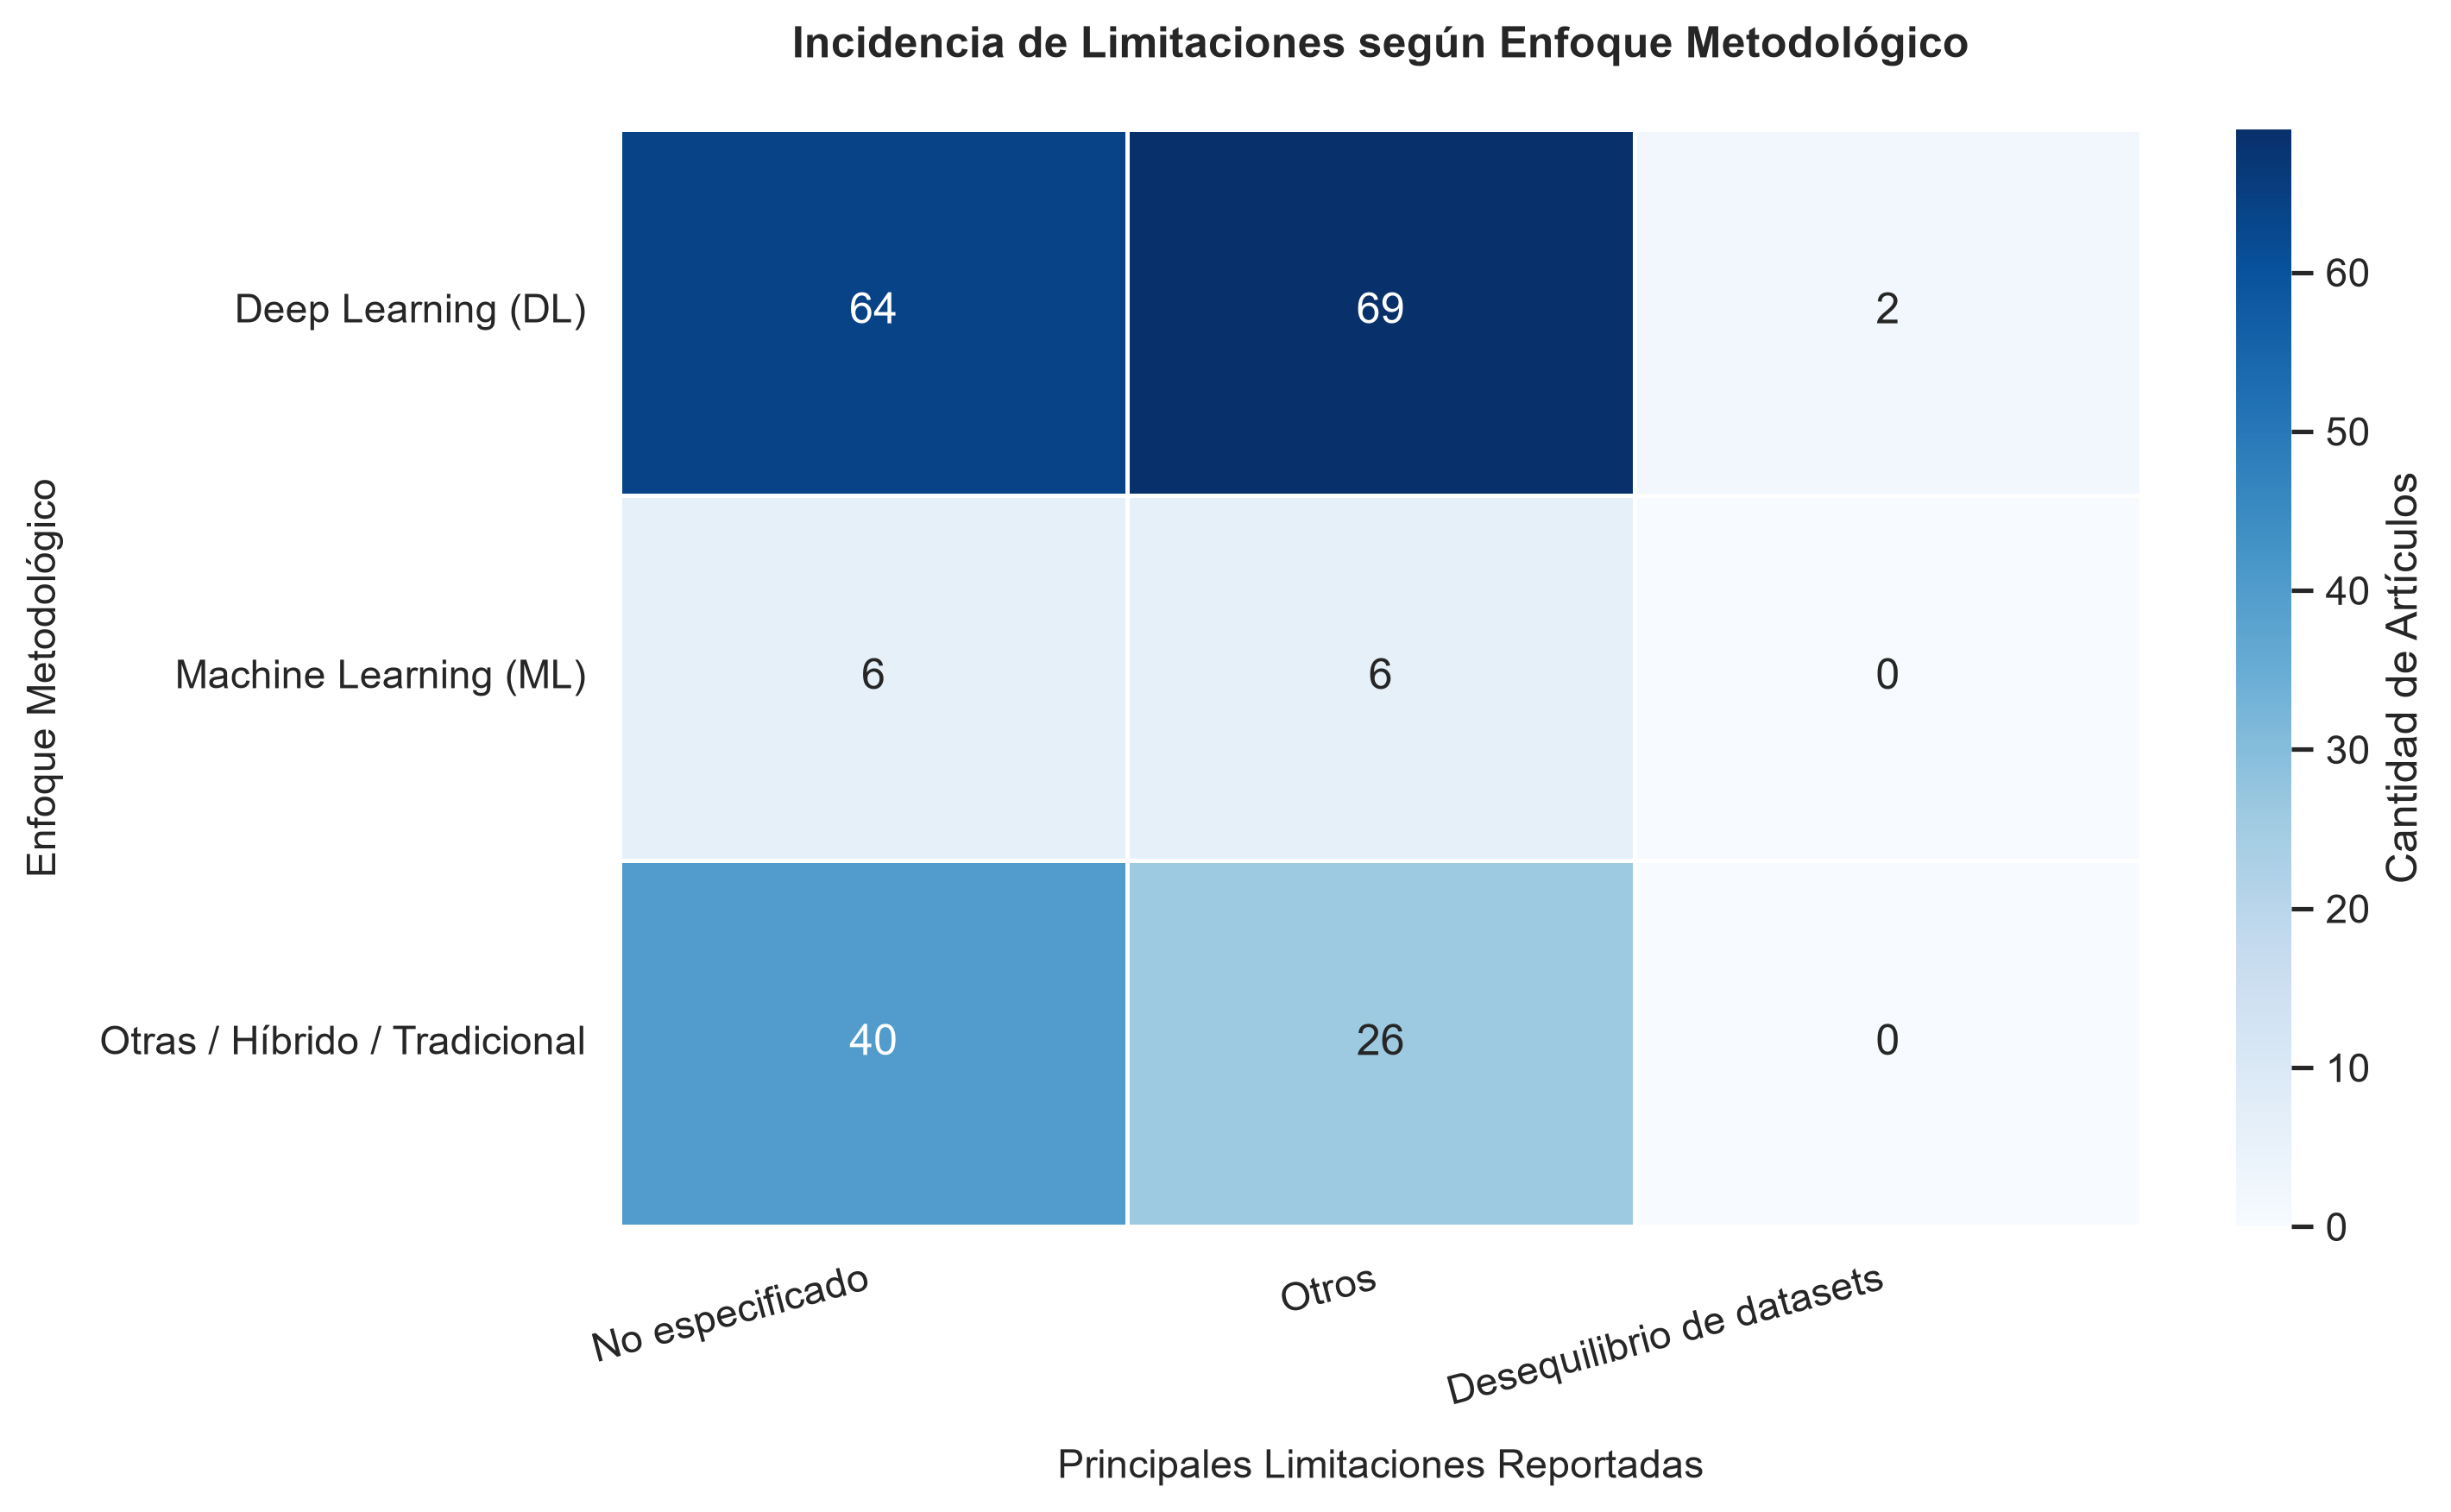
\includegraphics[width=0.48\textwidth]{../graficos/19_cruce_limitaciones_metodologia.png}}
\caption{Incidencia de Limitaciones según el Enfoque Metodológico de la Investigación.}
\label{fig:cruce_limitaciones}
\end{figure}

Para complementar esta perspectiva, la Fig.~\ref{fig:cruce_limitaciones_entorno} correlaciona la presencia de estos desafíos técnicos frente a los entornos de validación experimental. Se evidencia que los problemas de iluminación y la oclusión visual predominan en cámaras de circuito cerrado (CCTV) debido a factores climáticos descontrolados \cite{rachoti2025traffic, kumar2025smart}, mientras que la latencia y restricciones de hardware crítico representan los mayores obstáculos en el despliegue embebido a bordo y en vehículos aéreos (UAV) \cite{poudel2024improved, bakirci2024enhancing}.

\begin{figure}[htbp]
\centerline{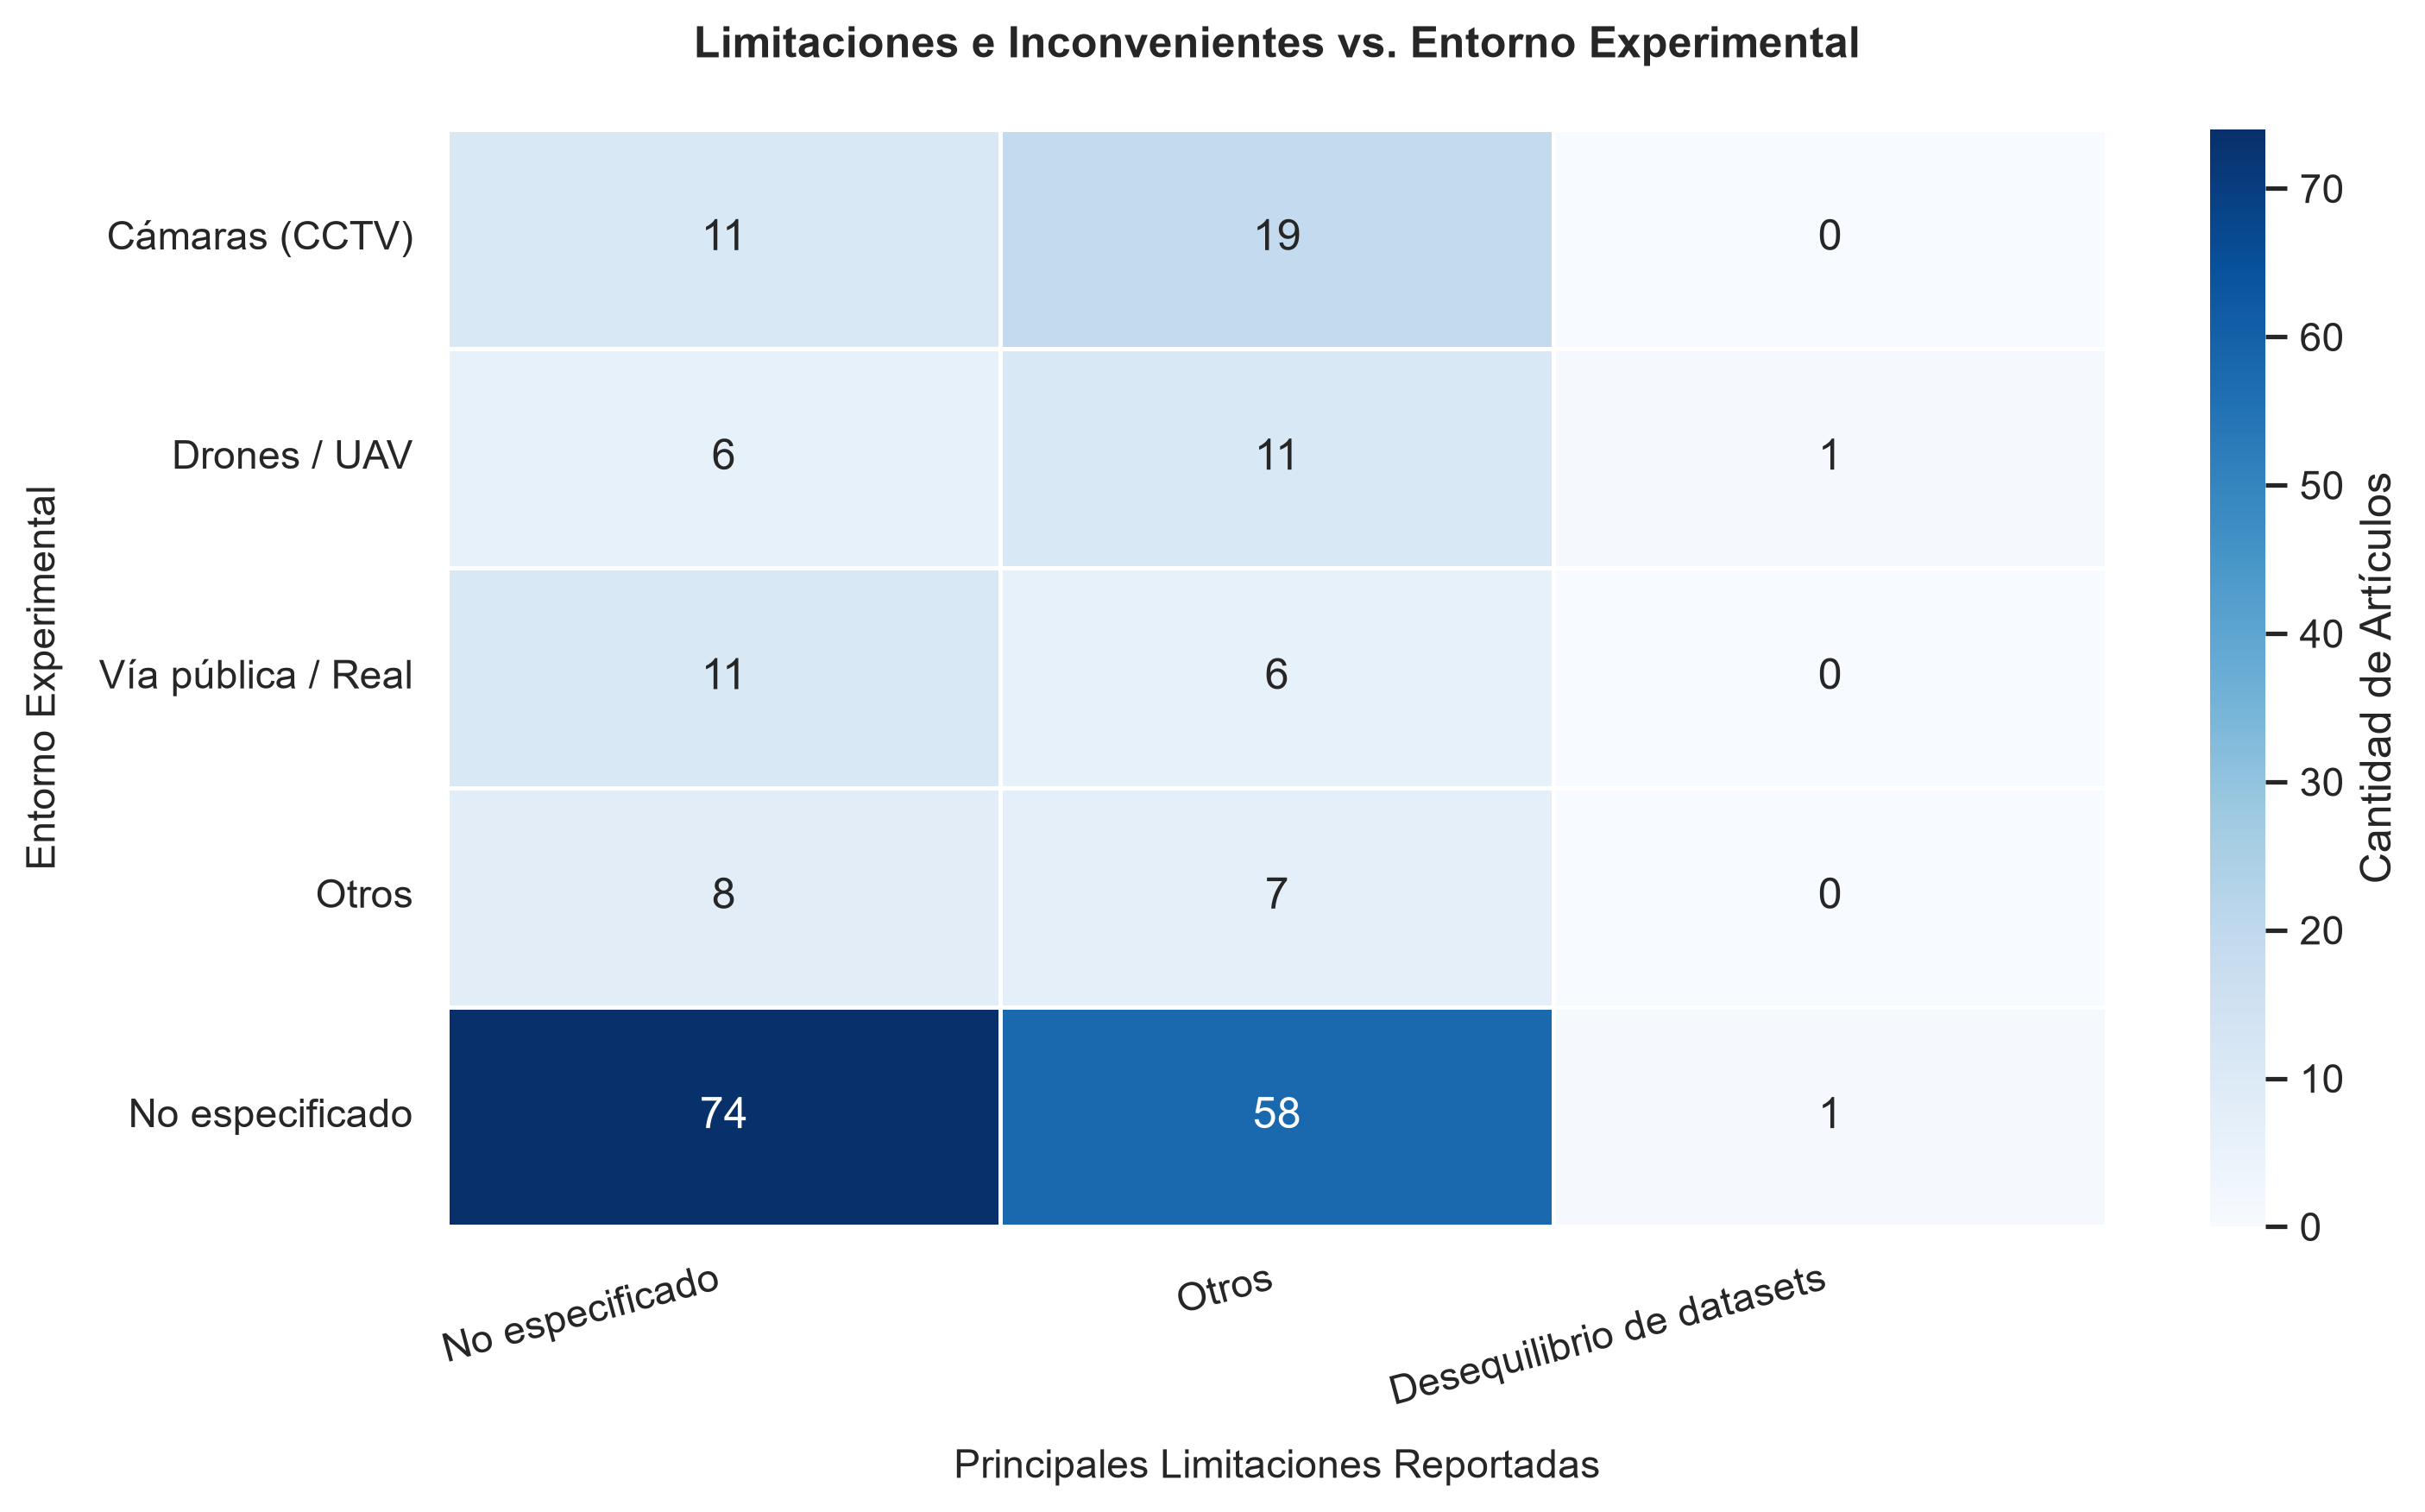
\includegraphics[width=0.48\textwidth]{../graficos/22_cruce_limitaciones_entorno.png}}
\caption{Correlación de Limitaciones e Inconvenientes vs. Entorno Experimental.}
\label{fig:cruce_limitaciones_entorno}
\end{figure}

\subsection{Desafíos de Privacidad, Ética y Seguridad de Datos}
El despliegue masivo de sistemas de monitoreo de conductores y cámaras de videovigilancia urbana plantea serios desafíos éticos y de privacidad de datos que deben ser abordados rigurosamente por los diseñadores de políticas públicas y desarrolladores de tecnología \cite{gowroju2025urbaneye, pujitha2025traffic}. La captura continua del rostro del conductor, el análisis de sus expresiones emocionales y el seguimiento de su mirada recopilan información biométrica de carácter altamente sensible. Si estos datos son transmitidos sin encriptación o almacenados de manera centralizada en servidores de la nube, se crea un riesgo latente de vulneración de la privacidad y acceso no autorizado por terceros \cite{balasaranya2025realtime, uddin2025abnormal}.

Normativas internacionales estrictas, como el Reglamento General de Protección de Datos (GDPR) en Europa, exigen que el procesamiento de datos biométricos se realice bajo principios de minimización de datos y consentimiento explícito. In respuesta a estos desafíos, la tendencia actual en el estado del arte se orienta fuertemente hacia el procesamiento en el borde (Edge Computing), donde la inferencia del modelo se ejecuta directamente dentro del hardware instalado en el vehículo (por ejemplo, microcontroladores avanzados o procesadores embebidos NVIDIA Jetson) \cite{nell2025classification, sorum2025modeling}. Al procesar las imágenes localmente y descartar de inmediato los fotogramas del video, transmitiendo únicamente alertas de metadatos (como "somnolencia detectada"), se resguarda de forma efectiva la identidad y privacidad del conductor, garantizando al mismo tiempo una baja latencia en la emisión de advertencias de seguridad.

Para mitigar los riesgos asociados con la transmisión de videos biométricos sensibles a servidores en la nube, el Aprendizaje Federado (Federated Learning) se posiciona como una solución altamente prometedora en la literatura reciente \cite{ijaradar2025datadriven, wang2025application}. Bajo este paradigma, los dispositivos embebidos en el borde a bordo de múltiples vehículos entrenan de forma colaborativa un modelo global compartiendo únicamente las actualizaciones de gradientes cifrados, sin exponer jamás la información biométrica cruda o el video del rostro a servidores centrales. Esto no solo garantiza el cumplimiento de normativas de privacidad rigurosas como la GDPR \cite{kumar2025smart, kalwa2025unusual}, sino que también reduce sustancialmente el ancho de banda necesario en redes móviles vehiculares (V2X).

\section{Conclusiones y Trabajo Futuro}
La presente revisión sistemática del estado del arte ha permitido evaluar de manera integral el desarrollo, madurez y desafíos actuales de las soluciones de visión computacional y aprendizaje automático aplicadas a los sistemas de transporte inteligentes y el monitoreo de conductores. A través del análisis estadístico cuantitativo del corpus de 213 publicaciones, se evidencia una consolidación científica significativa que está transformando el control y seguridad de nuestras redes viales.

Las conclusiones principales obtenidas de este análisis global son:
\begin{itemize}
    \item La hegemonía metodológica ha migrado casi en su totalidad hacia soluciones de Deep Learning debido a su alta capacidad de generalización en entornos urbanos dinámicos.
    \item El hardware embebido (Edge Computing) es fundamental para lograr implementaciones en tiempo real que garanticen la privacidad del conductor y baja latencia de procesamiento.
    \item Los desafíos actuales se centran en mitigar la sensibilidad de los modelos ante cambios climáticos y problemas de iluminación.
\end{itemize}

Como trabajo futuro, se vislumbran tres grandes áreas de desarrollo prioritarias en la literatura científica reciente:
\begin{enumerate}
    \item \textbf{Fusión de Sensores Multimodales:} La combinación de datos visuales con señales biométricas (EEG, ECG, conductancia de la piel) o datos espaciales (LiDAR, Radar) para robustecer la detección frente a oclusiones y cambios de iluminación.
    \item \textbf{Modelos de Lenguaje-Visión (Vision-Language Models) y Aprendizaje Zero-Shot:} La incorporación de arquitecturas multimedales que permitan detectar conductas atípicas de riesgo sin depender exclusivamente de clases predefinidas de entrenamiento.
    \item \textbf{Generación de Datos Sintéticos:} El uso de Redes Generativas Adversarias (GAN) y modelos de difusión para generar imágenes realistas de conducción nocturna, oclusiones y accidentes, resolviendo el problema de escasez de datos balanceados de entrenamiento.
\end{enumerate}


% Referencias bibliográficas
\nocite{*}
\printbibliography

\end{document}
